%\documentclass[a4paper,12pt,twoside]{book}
\documentclass[12pt,times]{report}
\usepackage{mathptmx}%This package supersedes times and mathptm
\usepackage[a4paper,right=2.54cm,left=2.54cm,top=2.54cm,bottom=2.54cm]{geometry}
\usepackage{float}
%%%%paquete para usar citas de diferentes formatos
%%%%%%%%%%%%%%%%%%%%%%%%%%%%%%%%%
%%add al indice
%\usepackage[nottoc,numbib]{tocbibind}
%\usepackage[authoryear,round]{natbib}
\usepackage[utf8]{inputenc}
\usepackage{csquotes}
\usepackage[spanish]{babel}
\usepackage[style=apa ,
%hyperref=auto,
%citestyle=authoryear,
natbib=true,
backend=biber]{biblatex}
\addbibresource{biblio/references.bib}
%\usepackage{biblatex}
%paquete para hiperlinks entre citas e imagenes
%%%%%%%%%%%%%%%%%%%%%%%%%%%%%%%%%
\usepackage[colorlinks=true,
citecolor=blue,
urlcolor=cyan,
bookmarks=true,
linkcolor=blue,
pdftitle={Tesis-nombre-alumno},
pdfauthor={autor nombres}]{hyperref}

\usepackage{amssymb}
\usepackage{graphicx} % for improved inclusion of graphics
%\usepackage{wrapfig} % to include figure with text wrapping around it
\usepackage[margin=10pt,font=small,labelfont=bf]{caption} % for improved layout of figure captions with extra margin, smaller font than text
\usepackage{eucal}
\usepackage[usenames, dvipsnames]{color}
\usepackage[perpage]{footmisc}
%\usepackage[round, sort]{natbib}
\usepackage{ifthen}
\usepackage{multicol} % for pages with multiple text columns, e.g. References
\setlength{\columnsep}{20pt} % space between columns; default 10pt quite narrow
\usepackage[nottoc]{tocbibind} % correct page numbers for bib in TOC, nottoc suppresses an entry for TOC itself
\usepackage{appendix}

%%%----Modificar encabezado y pie de pagina
%%%%%%%%%%%%%%%%%%%%%%%%%%%%%%%%%%%%%%%%%%%%%%%%%%%%%%%%%%%%%%%%%%%%%
\usepackage{fancyhdr} % for better header layout
\newcommand{\changefont}{%
	\fontsize{9pt}{1.5pt}\selectfont
}
\pagestyle{fancy}
\fancyhf{} %% delete default configuration of page
%%\setlength\headheight{15pt}
\fancyhead[L]{\changefont Titulo de tesis aqui}
\fancyhead[R]{\changefont \leftmark}
%%\fancyfoot[L]{\leftmark}
\fancyfoot[R]{\thepage}

%%%%%%%%%%%%%%%%%%%%%%%%%%%%%5
%%%% Configuracion de los parrafos
%\usepackage{setspace}
%\onehalfspacing
%\linespread{1.25} 
\setlength{\parindent}{0.5in} %%sangria
\setlength{\parskip}{3mm}  %%espacio entre parrafos
\linespread{1.3} %This equals 1.5 linespacing in Word
%%%% nuevo parrafo
%%%%%%%%%%%%%%%%%%%%%%%%%%%%%5
%%%% Centrar valores de una tabla
\usepackage{array}
%%CENTRADO HORIZONTAL
\newcolumntype{P}[1]{>{\centering\arraybackslash}p{#1}}
%%CENTRADO VERTICAL
\newcolumntype{M}[1]{>{\centering\arraybackslash}m{#1}}

%%%%%%%%%%%%%%%%%%%%%%%%%%%%%5
%%%%Paquete para alinear texto
\usepackage{ragged2e}
\usepackage{multirow}
\usepackage{makecell}
\usepackage{rotating}
\usepackage{siunitx} % To align the numbers later on
\usepackage[table,xcdraw]{xcolor}
\usepackage{color, colortbl}
\definecolor{Gray}{gray}{0.9}
\definecolor{orange}{rgb}{1,0.647,0}
\definecolor{turq3}{rgb}{0.54, 0.81, 0.94}
\definecolor{turq}{rgb}{0.63, 0.79, 0.95}
\definecolor{bluejean}{rgb}{0.03, 0.27, 0.49}

%%%%%%%%%%%%%%%%%%%%%%%%%
\usepackage{xparse}
\usepackage{expl3}
%%%%funcion de reemplazar regex
\ExplSyntaxOn
\NewDocumentCommand{\replace}{mmm}
{
	\marian_replace:nnn {#1} {#2} {#3}
}

\tl_new:N \l_marian_input_text_tl
\tl_new:N \l_marian_search_tl
\tl_new:N \l_marian_replace_tl

\cs_new_protected:Npn \marian_replace:nnn #1 #2 #3
{
	\tl_set:Nn \l_marian_input_text_tl { #1 }
	\tl_set:Nn \l_marian_search_tl { #2 }
	\tl_set:Nn \l_marian_replace_tl { #3 }
	\regex_replace_all:nnN { \b\u{l_marian_search_tl}\b } { \u{l_marian_replace_tl} } \l_marian_input_text_tl
	\tl_use:N \l_marian_input_text_tl
}
\ExplSyntaxOff

%%%%%%%%%%%%%%%%%%%%%%%%%%%%%%%%%%%%%%
\usepackage{amsmath}
\numberwithin{equation}{chapter} %%enumerar ecuaciones
\renewcommand{\theequation}{Ecuación \thechapter.\arabic{equation}}   
\usepackage{mathtools, nccmath, cool}
%%%Configuraciones de biblatex

%%%hel
%%%%\citeauthor
\makeatletter

%%%%%%%%%%%%
\DeclareCiteCommand{\citeauthor}
{\boolfalse{citetracker}%
	\boolfalse{pagetracker}%
	\usebibmacro{prenote}}
{\ifciteindex
	{\indexnames{labelname}}
	{}%
	\printtext[bibhyperref]{\printnames{labelname}}}
{\multicitedelim}
{\usebibmacro{postnote}}


\DeclareCiteCommand{\citetitle}
{\boolfalse{citetracker}%
	\boolfalse{pagetracker}%
	\usebibmacro{prenote}}
{\ifciteindex
	{\indexfield{indextitle}}
	{}%
	\printtext[bibhyperref]{\printfield[citetitle]{labeltitle}}}
{\multicitedelim}
{\usebibmacro{postnote}}

\DeclareCiteCommand{\cite}
{\usebibmacro{prenote}}
{\usebibmacro{citeindex}%
	\printtext[bibhyperref]{\usebibmacro{cite}}}
{\multicitedelim}
{\usebibmacro{postnote}}

\DeclareCiteCommand*{\cite}
{\usebibmacro{prenote}}
{\usebibmacro{citeindex}%
	\printtext[bibhyperref]{\usebibmacro{citeyear}}}
{\multicitedelim}
{\usebibmacro{postnote}}

\DeclareCiteCommand{\parencite}[\mkbibparens]
{\usebibmacro{prenote}}
{\usebibmacro{citeindex}%
	\printtext[bibhyperref]{\usebibmacro{cite}}}
{\multicitedelim}
{\usebibmacro{postnote}}

\DeclareCiteCommand*{\parencite}[\mkbibparens]
{\usebibmacro{prenote}}
{\usebibmacro{citeindex}%
	\printtext[bibhyperref]{\usebibmacro{citeyear}}}
{\multicitedelim}
{\usebibmacro{postnote}}

\DeclareCiteCommand{\footcite}[\mkbibfootnote]
{\usebibmacro{prenote}}
{\usebibmacro{citeindex}%
	\printtext[bibhyperref]{ \usebibmacro{cite}}}
{\multicitedelim}
{\usebibmacro{postnote}}

\DeclareCiteCommand{\footcitetext}[\mkbibfootnotetext]
{\usebibmacro{prenote}}
{\usebibmacro{citeindex}%
	\printtext[bibhyperref]{\usebibmacro{cite}}}
{\multicitedelim}
{\usebibmacro{postnote}}

\DeclareCiteCommand{\textcite}
{\boolfalse{cbx:parens}}
{\usebibmacro{citeindex}%
	\printtext[bibhyperref]{\usebibmacro{textcite}}}
{\ifbool{cbx:parens}
	{\bibcloseparen\global\boolfalse{cbx:parens}}
	{}%
	\multicitedelim}
{\usebibmacro{textcite:postnote}}
\makeatother
\makeatletter
\let\abx@macro@citeOrig\abx@macro@cite
\renewbibmacro{cite}{%
	\bibhyperref{%
		\let\bibhyperref\relax\relax%
		\abx@macro@citeOrig%
	}%
}
\let\abx@macro@textciteOrig\abx@macro@textcite
\renewbibmacro{textcite}{%
	\bibhyperref{%
		\let\bibhyperref\relax\relax%
		\abx@macro@textciteOrig%
	}%
}%

\makeatother

%%%%%%%%%%%%%%%%%%%%%%%%%%%%%%%%%%%%%%%%%%%
\begin{document}

\begin{titlepage}

	\begin{center}
		%%%cargar imagen
	    
\includegraphics[width=0.45\textwidth]{images_repo/esanlogomin}
		\vspace*{2cm} \\
		UNIVERSIDAD ESAN \vspace*{1ex} \\
		FACULTAD DE INGENIERÍA \vspace*{1ex} \\
		INGENIERÍA DE TECNOLOGÍAS DE INFORMACIÓN Y SISTEMAS\vspace*{8ex} \\
		\textbf{Sistema de Recomendación para la Distribución de Productos de Tiendas Retail mediante Visión por Computadora}
		\vspace*{8ex}\\	
		Trabajo de investigación para el curso de Trabajo de Tesis I 
		\vspace*{8ex} \\	
		Nombres alumnos: Alexis Meza and Neil Sanchez \\
		Asesor: Marks Calderón		
		\vfill
		
		Lima, \today 
		
	\end{center}
\end{titlepage}
%%cambiar nombres de objetos para el indice y otros
\renewcommand{\listfigurename}{Índice de Figuras}
\renewcommand{\tablename}{Tabla}
\renewcommand{\listtablename}{Índice de Tablas}

\thispagestyle{plain}
\begin{center}
	\vspace*{1.5cm}
	{\Large \bfseries  Resumen}
\end{center}
\vspace{0.5cm}

\newline

\textbf{Palabras claves: } uno, dos, tres, cuatro
\thispagestyle{plain}
\begin{center}
	\vspace*{1.5cm}
	{\Large \bfseries  Abstract}
\end{center}
\vspace{0.5cm}

\newline

\textbf{Keywords: } uno, dos, tres, cuatro
\thispagestyle{plain}
\begin{center}
	\vspace*{1.5cm}
	{\Large Para mi X, Y,X}
\end{center}


\thispagestyle{plain}
\begin{center}
	\vspace*{1.5cm}
	{\Large \bfseries  Agradecimientos}
\end{center}
\vspace{0.5cm}

\newline



% outline
\tableofcontents            % print the table of contents

%: ----------------------- contents ------------------------

\setcounter{secnumdepth}{3} % organisational level that receives a numbers
\setcounter{tocdepth}{3}    % print table of contents for level 3

% levels are: 0 - chapter, 1 - section, 2 - subsection, 3 - subsection


%: ----------------------- list of figures/tables ------------------------

\listoffigures	% print list of figures

\listoftables  % print list of tables



\chapter{PLANTEAMIENTO DEL PROBLEMA}
\section{Descripción de la Realidad Problemática}


El diseño de tiendas es un aspecto crucial para el éxito de cualquier negocio minorista. Además, las empresas de retail enfrentan una necesidad imperiosa de innovar para mantenerse competitivas. Muchos de estos negocios se enfrentaron a problemas importantes, como cierres obligatorios, una disminución de la demanda y problemas financieros. Según McKinsey, las tiendas minoristas pierden alrededor del 12-15\% de sus ingresos anuales debido a problemas como la falta de productos y exceso de inventario.

Las pequeñas y medianas tiendas, como los negocios retail familiares, suelen depender de procesos manuales para controlar su inventario y realizar la distribución de productos en el espacio de ventas. Según el Global Supply Chain Institute, el 53\% de los consumidores no completan su compra si el producto no está disponible en ese momento. Además, un estudio de Harvard Business Review menciona que aproximadamente el 70\% de los clientes que no encuentran el producto que buscan optan por no comprar en esa tienda, lo que se traduce en pérdidas considerables.

Sin embargo, también ha surgido un espíritu de resiliencia y renovación en el sector de los negocios pequeños a medida que el mundo se ha adaptado a la nueva realidad. Estos emprendedores han logrado reinventarse y encontrar nuevas oportunidades en el entorno empresarial debido a la creación de estrategias innovadoras y una mayor adopción de la tecnología.

Aquí es donde entra en juego las técnicas de visión por computadora, las cuales han demostrado ser herramientas efectivas para optimizar y mejorar la distribución de los productos en las tiendas. Además, la automatización de estos procesos mediante IA no solo reduciría costos operativos, sino que también aumentaría la eficiencia y la satisfacción del cliente. En la actualidad existen empresas que utilizan la visión por computadora, tales como Walmart, que ha implementado sistemas de IA que analizan los datos de cámaras en sus tiendas para detectar cuándo los estantes se quedan vacíos, logrando una reducción del 30\% en problemas de desabastecimiento (Walmart Labs, 2022). Otro ejemplo es Amazon Go, que utiliza un sistema de cámaras basado en visión por computadora que permite monitorear en tiempo real los productos que los clientes toman de los estantes. Este modelo no solo elimina la necesidad de cajas registradoras, sino que también optimiza la distribución de productos en las tiendas.

A pesar de los avances tecnológicos en grandes retailers, los negocios retail familiares y pequeños comercios no suelen tener acceso a estas tecnologías debido a costos elevados y falta de conocimientos técnicos. Según el estudio de Small Business Trends, el 45\% de los propietarios de pequeñas tiendas mencionan que la falta de recursos tecnológicos afecta significativamente su capacidad para competir con grandes retailers. La implementación de un sistema accesible que aproveche la visión por computadora puede ser una solución eficiente para automatizar el control de productos en estos comercios, mejorando su competitividad. Además, un reporte de Grand View Research indica que la adopción de inteligencia artificial en pymes crecerá a una tasa del 29.6\% entre 2021 y 2028, impulsada por la disponibilidad de soluciones más asequibles y específicas para cada sector.

El negocio retail ''La Económica'' es el negocio pequeño seleccionado para la investigación. Un negocio retail es un tipo de negocio pequeño que se enfoca en la venta de una amplia gama de productos de consumo diario en un espacio limitado. Los negocios retail son tiendas minoristas que ofrecen una forma conveniente de satisfacer las necesidades básicas de la comunidad local. Se encuentran con frecuencia en zonas residenciales o cerca de zonas con alta afluencia de personas, como oficinas o escuelas.

Estos negocios tienen como característica principal su tamaño compacto y su enfoque en proporcionar una selección de productos netamente esenciales, como alimentos frescos, enlatados, productos de higiene personal, bebidas y artículos de primera necesidad. Los negocios retail suelen diferenciarse de los supermercados más grandes principalmente por el tamaño, pero ofrecen una mayor comodidad y acceso rápido a los productos de primera necesidad, lo que los convierte en una de las opciones más populares para compras urgentes o rápidas.

Finalmente, la incorporación de visión por computadora en la recomendación para la distribución de productos de tiendas retail representa un avance trascendental. Esta tecnología permitirá a los propietarios realizar modificaciones de manera sencilla, rápida y en tiempo real. La modificación de los productos es crucial, ya que libera a los empleados de tareas tediosas para que se centren en atención al público y, por ende, aumenten las probabilidades de mejorar la experiencia del cliente.





%\begin{figure}[h]
%	\begin{center}
%		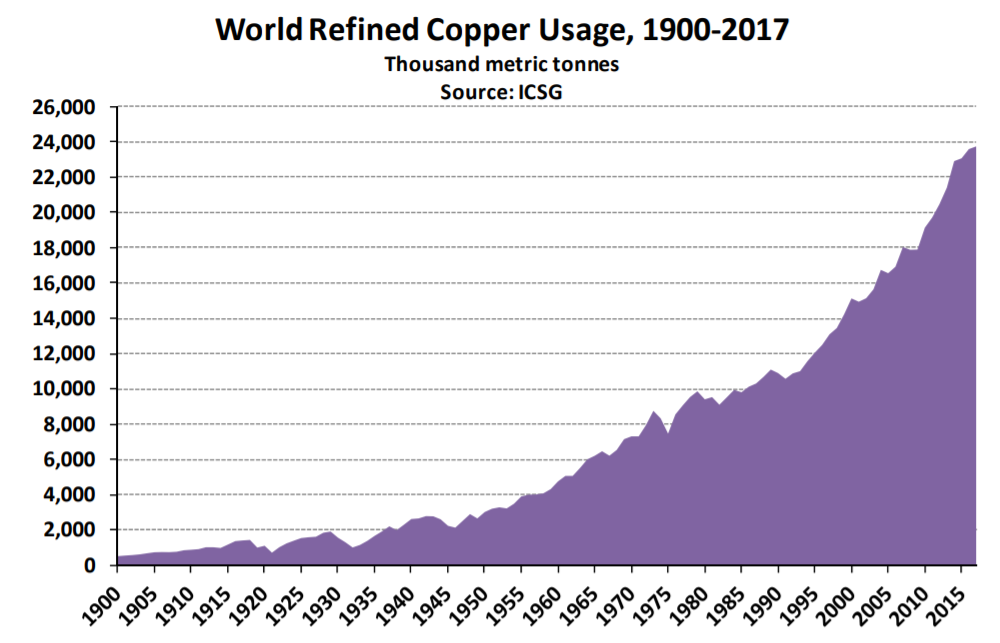
\includegraphics[width=0.8\textwidth]{1/figures/world_refined_copper_usage.png}
%		\caption{Uso del cobre refinado mundial del año 1900 a 2017 (en miles de toneladas). Fuente: \cite{cu_internationalcopper2018}}
%		\label{1:fig}
%	\end{center}
%\end{figure}

%\parencite{cu_internationalcopper2018}.





\section{Formulación del Problema}
Con el objetivo de formular los objetivos de esta investigación, se propusieron las siguientes preguntas.
\subsection{Problema General}
PG:\newcommand{\ProblemaGeneral}{
	¿Cómo el sistema de visión por computadora, que identifica clientes y analiza su comportamiento en una tienda retail, puede recomendar una mejor distribución de productos para optimizar el flujo de clientes y aumentar la eficiencia operativa en tiendas retail en el 2024?
}
\ProblemaGeneral
\subsection{Problemas Espec\'{i}ficos}
\newcommand{\Pbone}{
¿Qué técnicas de visión por computadora se deben usar para identificar y rastrear personas en tiempo real dentro de la tienda?
}
\newcommand{\Pbtwo}{
¿Qué métricas de comportamientos deben analizarse para detectar las zonas más y menos transitadas?
}
\newcommand{\Pbthree}{
¿Cómo debe estructurarse la arquitectura del sistema para procesar video y generar recomendaciones eficientemente?
}
\newcommand{\Pbfour}{
¿Cómo se puede medir el impacto del sistema en la eficiencia operativa y la experiencia del cliente?
}
%\newcommand{\Pbfive}{
%	ES
%}

\begin{itemize}
    \item PE1: {\Pbone}
	\item PE2: {\Pbtwo}
	\item PE3: {\Pbthree}
	\item PE4: {\Pbfour}
	%\item \Pbfive
\end{itemize}

\section{Objetivos de la Investigación}
El objetivo de esta investigación es ofrecer una solución tecnológica que permita a los retails mejorar su eficiencia operativa mediante la implementación de un sistema basado en visión por computadora. Este sistema proporcionará información en tiempo real sobre el comportamiento de los clientes, facilitando decisiones estratégicas para optimizar la disposición de productos, gestionar el inventario y asignar recursos de manera eficiente.
\subsection{Objetivo General}
OG:\newcommand{\ObjetivoGeneral}{
Desarrollar un sistema de visión por computadora que identifique y analice el comportamiento de los clientes dentro de una tienda retail, para recomendar una mejor distribución de productos, con el fin de optimizar el flujo de clientes, aumentar la eficiencia operativa y mejorar la experiencia de compra.
}
\ObjetivoGeneral
\subsection{Objetivos Espec\'{i}ficos}
\newcommand{\Objone}{
Identificar el mejor enfoque para detectar y rastrear personas en tiempo real con alta precisión.
}
\newcommand{\Objtwo}{
Determinar qué indicadores de movimiento y permanencia ayudan a identificar zonas transitadas y menos frecuentadas.
}
\newcommand{\Objthree}{
Definir una arquitectura que procese video y genere recomendaciones de manera rápida y eficiente.
}
\newcommand{\Objfour}{
Establecer métricas para evaluar mejoras en la eficiencia operativa y la satisfacción del cliente.
}
%\newcommand{\Objfive}{
%ghhhg
%}

\begin{itemize}
	\item OE1: {\Objone}
	\item OE2: {\Objtwo}
	\item OE3: {\Objthree}
	\item OE4: {\Objfour}
	%\item {\Objfive}
\end{itemize}

\section{Justificación de la Investigación}

\subsection{Teórica}
La visión por computadora ha emergido como una tecnología clave para automatizar tareas complejas en múltiples sectores, incluyendo el retail. Estudios previos han demostrado que técnicas de inteligencia artificial, como el reconocimiento de imágenes y el análisis de video, permiten identificar patrones de comportamiento en los consumidores y mejorar la disposición de productos en tiendas. Según investigaciones en el ámbito de la distribución minorista, una organización eficiente de los productos, basada en el análisis de datos visuales, puede incrementar las ventas y reducir el tiempo que un cliente invierte en encontrar productos . Además, la teoría de los sistemas recomendadores sugiere que combinar datos históricos de ventas y la interacción del cliente en tiempo real puede mejorar significativamente la satisfacción del cliente y la eficiencia operativa.
La presente investigación se justifica teóricamente porque amplía el conocimiento sobre el uso de la visión por computadora aplicada a entornos de retail familiar, donde la integración de estas tecnologías ha sido limitada por falta de recursos o conocimientos técnicos. Aportará un marco teórico sobre cómo los patrones de movimiento de los clientes, junto con los datos transaccionales, pueden generar recomendaciones dinámicas para la redistribución de productos en un espacio físico limitado.

\subsection{Práctica}
En el contexto de tiendas retail familiares, la implementación de tecnología avanzada, como la visión por computadora, puede transformar procesos actualmente manuales y propensos a errores. Al automatizar el monitoreo y la distribución de productos, las pequeñas tiendas pueden competir más eficazmente con grandes retailers que ya utilizan IA para optimizar sus operaciones. Investigaciones adicionales han demostrado que la optimización de la distribución de productos mediante el análisis del flujo de clientes puede aumentar las ventas hasta en un 15\%. Un estudio realizado por Walmart Labs en 2022 mostró que la aplicación de inteligencia artificial y visión por computadora permitió reducir en un 30\% los problemas de desabastecimiento en sus tiendas, lo que pone de manifiesto el impacto práctico de la tecnología en la optimización operativa. 

La investigación es necesaria para proporcionar una solución práctica y asequible a pequeños negocios que carecen de los recursos de grandes cadenas. Este proyecto de tesis también tiene un enfoque práctico en mejorar la experiencia del cliente al reducir los tiempos de espera y facilitar la disposición de productos más relevante en las zonas de mayor tránsito.

\subsection{Metodológica}. 
La metodología a emplear en esta investigación estará basada en el uso de técnicas de visión por computadora como YOLOv5 o RetinaNet para la detección en tiempo real de clientes dentro de la tienda. El análisis de video se procesará utilizando redes neuronales convolucionales, lo que permite identificar con precisión los patrones de comportamiento y flujo de los clientes. Además, se integrarán datos de ventas y stock en un sistema de recomendación basado en machine learning para sugerir la redistribución de productos. El enfoque metodológico garantiza que los resultados obtenidos sean aplicables no solo en "La Económica", sino también replicables en otros negocios retail de características similares.

La justificación metodológica de este proyecto radica en su innovación al combinar algoritmos de visión por computadora con técnicas de análisis de comportamiento del cliente y optimización de inventario en un solo sistema integrado.
\section{Delimitación del Estudio}
A continuación, se presentará la delimitación espacial, temporal y conceptual.
\subsection{Espacial}
El presente estudio se llevará a cabo en el negocio retail "La Económica", una pequeña tienda minorista ubicada en Lima, Perú. La selección de esta tienda responde a su representatividad dentro del contexto de los pequeños comercios familiares en zonas urbanas de alta densidad. Esta tienda tiene una disposición de productos que sigue un modelo tradicional de retail, pero enfrenta problemas en la gestión y distribución de inventario debido a la falta de recursos tecnológicos. El análisis de la implementación del sistema de visión por computadora se concentrará en este espacio físico, utilizando los datos de comportamiento de los clientes y las características del lugar para optimizar la distribución de productos.

\subsection{Temporal}
El periodo de investigación abarcará desde enero hasta diciembre de 2024. Este periodo permitirá realizar observaciones a lo largo de diferentes estaciones del año, teniendo en cuenta variaciones en el comportamiento del cliente debido a fechas festivas, promociones y cambios estacionales en la demanda de productos. Adicionalmente, se prevé un tiempo de implementación del sistema de visión por computadora, así como un periodo de adaptación para los empleados del negocio.

\subsection{Conceptual}
Para los fines de esta investigación, se definirán los siguientes conceptos clave:
\begin{itemize}
    \item \textbf{Visión por Computadora:} Tecnología que permite a las computadoras y sistemas interpretar y tomar decisiones basadas en imágenes visuales capturadas por cámaras, utilizando algoritmos avanzados de inteligencia artificial para identificar patrones y objetos en tiempo real.
    \item \textbf{Distribución de Productos:} La disposición y organización de los productos dentro de una tienda retail con el fin de optimizar el acceso de los clientes a los productos de mayor demanda y mejorar el flujo de clientes en el establecimiento.
    \item \textbf{Flujo de Clientes:} El patrón de movimiento de los consumidores dentro de la tienda, incluyendo las áreas más frecuentadas, tiempos de permanencia y rutas más comunes que siguen al recorrer el espacio de ventas.
    \item \textbf{Eficiencia Operativa:} La capacidad de un negocio para utilizar sus recursos (tiempo, espacio y personal) de manera óptima, minimizando costos y mejorando la calidad del servicio, lo cual incluye la correcta gestión de inventarios y la disposición eficiente de productos.
\end{itemize}


%\subsection{Matriz de Consistencia}
%A continuación se presenta la matriz de consistencia elaborada para la presente investigación (véase Anexo \ref{1:table}).


\chapter{MARCO TEÓRICO}
\section{Antecedentes de la investigación}
A continuación, en esta sección se presentarán 10 artículos de investigación las cuales abordarán diversas técnicas y enfoques que se emplearon para afrontar problemas similares al de esta tesis. Es importante señalar que hasta la fecha
 no se ha encontrado investigación alguna sobre este tema a nivel nacional. Asimismo, a continuación se presenta un cuadro resumen (véase Anexo \ref{A:table}) de lo que se presenta en esta sección.



\subsection{A novel low-resource consumption and high-speed hardware implementation of HOG feature extraction on FPGA for human detection }


\subsubsection{Planteamiento del Problema y objetivo }
El artículo se enfoca en la creciente necesidad de mejorar la detección de peatones en entornos de tráfico complejos, dada la importancia de garantizar la seguridad de los transeúntes y la fluidez del tráfico. La implementación de algoritmos de detección de peatones en vehículos inteligentes tiene un impacto significativo en la reducción de accidentes y la optimización del flujo vehicular. Sin embargo, el desarrollo de estos sistemas presenta desafíos considerables, especialmente cuando se requieren soluciones que sean tanto eficientes en términos de precisión como de consumo de recursos computacionales. Los métodos tradicionales basados en redes neuronales convolucionales (CNN) han demostrado ser eficaces, pero su adopción en dispositivos con recursos limitados, como los sistemas embebidos en vehículos, se ve restringida debido a sus elevadas demandas computacionales. Por ello, el objetivo del estudio es diseñar una implementación optimizada del algoritmo Histogramas de Gradientes Orientados (HOG) en hardware utilizando FPGA (Field Programmable Gate Array), con el fin de reducir el uso de recursos y aumentar la velocidad de procesamiento, sacrificando mínimamente la precisión del sistema.

\subsubsection{Técnicas empleadas por los autores}
Los autores han propuesto varias técnicas para optimizar la implementación del algoritmo HOG en hardware. Una de las técnicas principales consiste en la simplificación del cálculo de la magnitud y orientación de los gradientes, reduciendo la cantidad de operaciones computacionales requeridas. Tradicionalmente, la asignación de bins en el algoritmo HOG se realiza mediante funciones trigonométricas como la arcotangente, lo que incrementa el costo computacional. En este estudio, los autores han desarrollado un método alternativo basado en comparaciones que evita el uso de funciones trigonométricas. En lugar de calcular el ángulo exacto del vector de gradiente, el rango de 0 a 180 grados se divide en 8 bins de 22.5 grados cada uno, permitiendo una asignación rápida a través de comparaciones sucesivas de las magnitudes y signos de los gradientes en las direcciones x y. Para el cálculo de la magnitud del gradiente, en lugar de utilizar la fórmula exacta que implica operaciones de raíz cuadrada, se implementa una aproximación que utiliza comparaciones y multiplicaciones predefinidas, lo que reduce significativamente la utilización de unidades de procesamiento de señales digitales (DSP). Asimismo, para la normalización de bloques, se opta por la aproximación de Newton-Raphson para el cálculo de la inversa de la raíz cuadrada, lo cual reduce el uso de hardware especializado y acelera el proceso.

\subsubsection{Metodología empleada por los autores}
La implementación del sistema se llevó a cabo utilizando un FPGA Xilinx Artix-7, seleccionado por su capacidad para soportar operaciones en paralelo, un aspecto crítico para mejorar la eficiencia del algoritmo HOG en tiempo real. El flujo de trabajo inicia con la conversión de la imagen de entrada al formato de escala de grises, lo que simplifica el proceso de cálculo de gradientes. A continuación, se utiliza el operador Sobel para determinar los gradientes en las direcciones 
 x y, lo que permite detectar cambios significativos en la intensidad de la imagen. La técnica de asignación de bins se implementa mediante una jerarquía de comparaciones: primero se evalúa el signo del gradiente en la dirección x, seguido de la comparación de las magnitudes relativas de los componentes x y, y finalmente se aplica un umbral para determinar el bin exacto. Esta técnica minimiza el uso de recursos, ya que requiere solo tres comparaciones y una multiplicación. Para la etapa de normalización, el enfoque basado en Newton-Raphson permite aproximar la raíz cuadrada inversa de manera eficiente, empleando un valor inicial calculado que reduce el número de iteraciones necesarias. Los histogramas de gradientes se construyen para cada celda y luego se normalizan por bloques, lo que garantiza que los descriptores de características sean robustos frente a cambios en la iluminación de la imagen.
%%%Ecuacion
%\begin{equation}  
%\label{eq:RMSE}
%RMSE = \sqrt{\frac{\sum_{i=1}^{N}{\Big(O_i -T_i\Big)^2}}{N}}
%\end{equation}


\subsubsection{Resultados obtenidos}
El diseño propuesto demostró una mejora sustancial en términos de consumo de recursos y velocidad de procesamiento comparado con las implementaciones tradicionales del algoritmo HOG en hardware. En particular, el sistema utilizó 4117 tablas de búsqueda (LUTs) y 4.5 Kbits de memoria RAM de bloque, lo que representa una reducción significativa respecto a otras implementaciones, algunas de las cuales superan los 10,000 LUTs y utilizan más de 300 Kbits de memoria. En cuanto a la velocidad de procesamiento, se alcanzó un rendimiento de 0.933 píxeles por ciclo de reloj, lo que supone una mejora considerable en comparación con otros métodos, que generalmente se encuentran en el rango de 0.4 a 0.7 píxeles por ciclo. En términos de precisión, el sistema mostró una reducción mínima, con una disminución del 1.2\% en la exactitud para el conjunto de datos INRIA y del 0.11\% para el conjunto de datos MIT. Aunque la precisión se vio ligeramente afectada, esta pérdida es aceptable en aplicaciones donde la eficiencia y el consumo de recursos son críticos. Las simulaciones realizadas en MATLAB mostraron una diferencia de precisión menor al 0.5\% respecto a la implementación en hardware, lo que subraya la fiabilidad del enfoque propuesto.


\subsection{Robust Human Detection Using Histogram
Oriented Gradient and Aggregate Channel}

\subsubsection{Planteamiento del Problema y objetivo }
El artículo aborda la creciente demanda en los sistemas de detección de objetos, particularmente en aplicaciones con vehículos autónomos y drones, en los cuales resulta fundamental una detección eficaz y precisa para la correcta operación de estas plataformas en tiempo real. Los sistemas de vigilancia, control de tráfico y los dispositivos autónomos requieren identificar y rastrear objetos con alta precisión, incluso bajo condiciones difíciles, como variaciones de iluminación o presencia de obstáculos. Sin embargo, los métodos tradicionales de redes neuronales profundas, aunque precisos, requieren de gran capacidad de procesamiento y un extenso conjunto de datos para su entrenamiento, lo que limita su aplicación en hardware con recursos limitados. Ante este desafío, el estudio tiene como objetivo desarrollar un sistema de detección de humanos que sea preciso y eficiente, basado en características de gradiente orientado (HOG) y características de canal agregado (ACF), complementado con una arquitectura de red neuronal convolucional (CNN) como GoogleNet. Esta integración tiene como propósito mejorar la precisión en la detección y reducir el consumo de recursos, haciéndolo ideal para plataformas de hardware limitado como vehículos autónomos y sistemas de búsqueda y rescate en ambientes adversos.



\subsubsection{Técnicas empleadas por los autores}
Para optimizar la eficiencia en la detección de humanos, los autores emplean una combinación de técnicas avanzadas. Se utiliza GoogleNet como un sistema de atención que filtra las imágenes que contienen objetivos humanos, optimizando así el uso de la CPU al evitar procesar imágenes irrelevantes. Esto se complementa con el uso de las características HOG y ACF. GoogleNet identifica eficazmente las imágenes de interés y las clasifica con una precisión del 99.69\%, minimizando la pérdida de información a un 0.05\%. Una vez identificadas las imágenes con presencia humana, el sistema utiliza ACF con un clasificador AdaBoost para optimizar la detección y clasificación de objetos en múltiples escalas, lo cual es adecuado para entornos de movimiento rápido. Además, el sistema fusiona estas características de gradiente y canal, reduciendo los errores de detección y mejorando la robustez frente a variaciones de fondo y condiciones de iluminación. Esta combinación de técnicas garantiza una alta precisión en las detecciones y reduce el tiempo de procesamiento de cada cuadro.

\subsubsection{Metodología empleada por los autores}
El sistema propuesto utiliza una metodología que combina diversas etapas de procesamiento en secuencia, apoyándose en múltiples modelos de CNN y técnicas de procesamiento de imágenes. Primero, se compararon varios modelos de CNN (ResNet18, ResNet50, SqueezeNet, Darknet53 y GoogleNet) en términos de precisión y pérdida, utilizando datos de los conjuntos UAV123, UAV123@10fps, COCO y OpenImagesV6. GoogleNet mostró el mejor rendimiento, con una precisión del 99.69\% y mínima pérdida, por lo cual fue seleccionado para la clasificación preliminar de imágenes con contenido humano. Una vez filtradas las imágenes relevantes, se aplican las características ACF y HOG mediante AdaBoost, lo que permite determinar las posiciones exactas de los objetivos en las imágenes detectadas. Para el entrenamiento del sistema, se empleó un total de 3252 imágenes, utilizando un 70\% para entrenamiento y un 30\% para validación, con un procesador Intel Core i5 y 8 GB de RAM. La configuración de los parámetros para los entrenamientos de CNN incluyó un tamaño de minibatch de 100, una tasa de aprendizaje inicial de 0.001 y un máximo de 10 épocas, buscando optimizar la precisión del sistema sin comprometer la eficiencia.
%%%Ecuacion
%\begin{equation}  
%\label{eq:RMSE}
%RMSE = \sqrt{\frac{\sum_{i=1}^{N}{\Big(O_i -T_i\Big)^2}}{N}}
%\end{equation}


\subsubsection{Resultados obtenidos}
Los resultados obtenidos en el estudio demuestran una mejora significativa en la precisión y eficiencia del sistema. Al combinar GoogleNet con ACF y HOG, el sistema alcanzó una precisión de 97.4\%, notablemente superior al 92.1\% logrado con GoogleNet y ACF sin HOG, y al 89\% utilizando únicamente ACF. La inclusión de HOG como complemento mejora considerablemente la detección de objetivos humanos en entornos con ruido o iluminación cambiante. En términos de velocidad de procesamiento, la propuesta reduce significativamente la carga en la CPU, alcanzando hasta un 75\% de ahorro al desactivar el procesamiento de imágenes irrelevantes. La velocidad de procesamiento en imágenes con presencia humana es de 5 cuadros por segundo (FPS), mientras que al desactivar las características de detección en imágenes sin humanos, la velocidad alcanza los 20 FPS. Estos resultados confirman la eficacia del sistema propuesto, que equilibra precisión y eficiencia, haciéndolo adecuado para aplicaciones en vehículos no tripulados y en sistemas de búsqueda y rescate en condiciones adversas.

\subsection{When AI meets store layout design: a review}
Nguyen, Le, Martin, Cil y Fookes publicaron un artículo en la revista Artificial Intelligence Review en el año 2022, titulado “When AI meets store layout design: a review”, que en español se traduce como “Cuando la inteligencia artificial se encuentra con el diseño de distribución en tiendas: una revisión”.

\subsubsection{Planteamiento del Problema y objetivo }
El artículo examina cómo la inteligencia artificial (IA) puede transformar el diseño de distribución de tiendas, optimizando la presentación de mercancías para captar la atención del cliente y mejorar la rentabilidad. Este tema es crucial, ya que un diseño eficiente de la tienda fomenta que los clientes exploren más pasillos y se expongan a una mayor cantidad de productos, lo cual se asocia directamente con el incremento en las ventas. Tradicionalmente, el diseño de las tiendas responde de manera pasiva al comportamiento del cliente, basándose en la observación de ventas y en cambios de exhibición para incrementar la demanda. Sin embargo, este enfoque tradicional no captura la navegación real de los clientes ni sus tiempos de estancia en cada sección. A través de la aplicación de la IA en la infraestructura de videovigilancia (CCTV) existente, este estudio busca proporcionar una nueva perspectiva que permita entender y predecir el comportamiento del cliente dentro de las tiendas. El objetivo del estudio es, entonces, realizar una revisión exhaustiva de los enfoques tradicionales y modernos, proponiendo un marco impulsado por IA que transforme datos de CCTV en inteligencia empresarial para mejorar el diseño de las tiendas.




\subsubsection{Técnicas empleadas por los autores}
Los autores emplean diversas técnicas de análisis de video e inteligencia artificial, destacando el uso de técnicas de visión computacional y aprendizaje profundo para captar y analizar el comportamiento del cliente. Utilizan métodos de reconocimiento de patrones y detección de objetos, incluidos algoritmos de detección de rostros y reconocimiento emocional, que permiten identificar la disposición emocional de los clientes frente a los productos exhibidos. Estas técnicas de IA se aplican sobre los datos capturados por CCTV, permitiendo así un análisis detallado del flujo de clientes, la identificación de los productos que captan mayor atención y la detección de zonas con baja interacción. Además, los autores incorporan técnicas de analítica avanzada, como mapas de calor, que visualizan las áreas de mayor tráfico y el tiempo que los clientes dedican a diferentes secciones de la tienda. Estas técnicas proporcionan una comprensión profunda y cuantitativa del comportamiento del cliente, ofreciendo bases para rediseñar la distribución de los espacios de manera informada.


\subsubsection{Metodología empleada por los autores}
La metodología del estudio se estructura en un marco denominado “Sense-Think-Act-Learn” (STAL), que divide el proceso en cuatro etapas: 1) Captura de datos mediante la recopilación de videos de CCTV y otros datos de mercado, 2) Procesamiento de datos utilizando técnicas de analítica de video para limpiar, transformar y de-identificar la información respetando la privacidad de los clientes, 3) Análisis inteligente de video mediante el cual algoritmos de IA analizan patrones de comportamiento y preferencias de los clientes en tiempo real, y 4) Toma de decisiones donde los resultados de la analítica se implementan para optimizar el diseño de la tienda y mejorar la satisfacción del cliente. Este marco metodológico permite una evaluación continua, que facilita la reestructuración de los espacios de la tienda según los patrones de tráfico y las preferencias observadas. El sistema es escalable, al utilizar un sistema en la nube que permite almacenar y analizar grandes volúmenes de datos sin los costos de mantenimiento asociados a sistemas locales.

%%%Ecuacion
%\begin{equation}  
%\label{eq:RMSE}
%RMSE = \sqrt{\frac{\sum_{i=1}^{N}{\Big(O_i -T_i\Big)^2}}{N}}
%\end{equation}


\subsubsection{Resultados obtenidos}
Los resultados obtenidos con la implementación del marco propuesto reflejan una mejora significativa en la optimización de la distribución de tiendas y en la satisfacción del cliente. El análisis de datos de video, en conjunto con mapas de calor y técnicas de reconocimiento de emociones, permite identificar patrones de navegación y zonas de alta interacción. Esto ha demostrado ser efectivo para ubicar productos estratégicamente y reorganizar el espacio de manera que maximice la exposición de mercancías populares y optimice la experiencia de compra. El estudio muestra que la implementación de un sistema basado en IA permite aumentar la eficiencia en la gestión de inventarios y en la planificación de la tienda, mejorando las métricas de rendimiento como el tiempo de estancia de los clientes en la tienda y el flujo de tráfico. Este enfoque integral orientado a la satisfacción del cliente y la eficiencia operacional presenta una base sólida para futuras investigaciones y aplicaciones en la optimización de tiendas mediante IA.


\subsection{Utilizing Gen AI and Computer Vision for Applications in the Retail}
Nguyen, Le, Martin, Cil y Fookes publicaron un artículo en la revista Artificial Intelligence Review en el año 2022, titulado “When AI meets store layout design: a review”, que en español se traduce como “Cuando la inteligencia artificial se encuentra con el diseño de distribución en tiendas: una revisión”.

\subsubsection{Planteamiento del Problema y objetivo }
El artículo examina cómo la inteligencia artificial (IA) puede transformar el diseño de distribución de tiendas, optimizando la presentación de mercancías para captar la atención del cliente y mejorar la rentabilidad. Este tema es crucial, ya que un diseño eficiente de la tienda fomenta que los clientes exploren más pasillos y se expongan a una mayor cantidad de productos, lo cual se asocia directamente con el incremento en las ventas. Tradicionalmente, el diseño de las tiendas responde de manera pasiva al comportamiento del cliente, basándose en la observación de ventas y en cambios de exhibición para incrementar la demanda. Sin embargo, este enfoque tradicional no captura la navegación real de los clientes ni sus tiempos de estancia en cada sección. A través de la aplicación de la IA en la infraestructura de videovigilancia (CCTV) existente, este estudio busca proporcionar una nueva perspectiva que permita entender y predecir el comportamiento del cliente dentro de las tiendas. El objetivo del estudio es, entonces, realizar una revisión exhaustiva de los enfoques tradicionales y modernos, proponiendo un marco impulsado por IA que transforme datos de CCTV en inteligencia empresarial para mejorar el diseño de las tiendas.




\subsubsection{Técnicas empleadas por los autores}
Los autores emplean diversas técnicas de análisis de video e inteligencia artificial, destacando el uso de técnicas de visión computacional y aprendizaje profundo para captar y analizar el comportamiento del cliente. Utilizan métodos de reconocimiento de patrones y detección de objetos, incluidos algoritmos de detección de rostros y reconocimiento emocional, que permiten identificar la disposición emocional de los clientes frente a los productos exhibidos. Estas técnicas de IA se aplican sobre los datos capturados por CCTV, permitiendo así un análisis detallado del flujo de clientes, la identificación de los productos que captan mayor atención y la detección de zonas con baja interacción. Además, los autores incorporan técnicas de analítica avanzada, como mapas de calor, que visualizan las áreas de mayor tráfico y el tiempo que los clientes dedican a diferentes secciones de la tienda. Estas técnicas proporcionan una comprensión profunda y cuantitativa del comportamiento del cliente, ofreciendo bases para rediseñar la distribución de los espacios de manera informada.


\subsubsection{Metodología empleada por los autores}
La metodología del estudio se estructura en un marco denominado “Sense-Think-Act-Learn” (STAL), que divide el proceso en cuatro etapas: 1) Captura de datos mediante la recopilación de videos de CCTV y otros datos de mercado, 2) Procesamiento de datos utilizando técnicas de analítica de video para limpiar, transformar y de-identificar la información respetando la privacidad de los clientes, 3) Análisis inteligente de video mediante el cual algoritmos de IA analizan patrones de comportamiento y preferencias de los clientes en tiempo real, y 4) Toma de decisiones donde los resultados de la analítica se implementan para optimizar el diseño de la tienda y mejorar la satisfacción del cliente. Este marco metodológico permite una evaluación continua, que facilita la reestructuración de los espacios de la tienda según los patrones de tráfico y las preferencias observadas. El sistema es escalable, al utilizar un sistema en la nube que permite almacenar y analizar grandes volúmenes de datos sin los costos de mantenimiento asociados a sistemas locales.

%%%Ecuacion
%\begin{equation}  
%\label{eq:RMSE}
%RMSE = \sqrt{\frac{\sum_{i=1}^{N}{\Big(O_i -T_i\Big)^2}}{N}}
%\end{equation}


\subsubsection{Resultados obtenidos}
Los resultados obtenidos con la implementación del marco propuesto reflejan una mejora significativa en la optimización de la distribución de tiendas y en la satisfacción del cliente. El análisis de datos de video, en conjunto con mapas de calor y técnicas de reconocimiento de emociones, permite identificar patrones de navegación y zonas de alta interacción. Esto ha demostrado ser efectivo para ubicar productos estratégicamente y reorganizar el espacio de manera que maximice la exposición de mercancías populares y optimice la experiencia de compra. El estudio muestra que la implementación de un sistema basado en IA permite aumentar la eficiencia en la gestión de inventarios y en la planificación de la tienda, mejorando las métricas de rendimiento como el tiempo de estancia de los clientes en la tienda y el flujo de tráfico. Este enfoque integral orientado a la satisfacción del cliente y la eficiencia operacional presenta una base sólida para futuras investigaciones y aplicaciones en la optimización de tiendas mediante IA.

\subsection{Análisis del comportamiento de clientes mediante detección de personas}

Este artículo presenta un framework para analizar el comportamiento de clientes en tiendas minoristas mediante la detección de personas en videos de vigilancia. Se desarrolla un pipeline que aplica el modelo SiamMOT para el seguimiento de personas, complementado por un proceso de pre y postprocesamiento. Los resultados brindan información útil para el negocio, como indicadores y mapas de calor de las zonas ocupadas, y se valida mediante comparación manual para evaluar la precisión del algoritmo.



\subsubsection{Planteamiento del Problema y objetivo }
El artículo se enfoca en resolver la dificultad que enfrentan los algoritmos tradicionales de detección de personas al ser implementados en entornos comerciales reales, donde las condiciones de operación son complejas debido a la presencia de obstáculos físicos (mesas, góndolas, carteles) y oclusiones entre clientes, además de variaciones de luz y ruido en la imagen . Según estudios recientes, más del 70\% de las personas en videos tomados en tiendas y bancos aparecen parcialmente ocluidas, lo que reduce la eficacia de los métodos convencionales de detección. Ante esta situación, los sistemas de seguimiento basados en aprendizaje profundo, como las redes neuronales convolucionales (CNN), han demostrado una mayor eficacia, pero requieren alto poder computacional, lo que limita su implementación en hardware accesible para pequeños comercios.

Por lo tanto, este trabajo propone el desarrollo de un framework eficiente para detectar y seguir personas en tiempo real, optimizado para funcionar en sistemas con recursos limitados, como computadoras de uso doméstico. El objetivo principal es proveer herramientas de análisis, como mapas de calor y conteos de aforo en cada momento, que puedan ser utilizados por los negocios para mejorar la gestión de espacios y comprender el comportamiento de la clientela.



\subsubsection{Técnicas empleadas por los autores}
El enfoque propuesto utiliza el modelo SiamMOT (Siamese Multi-Object Tracking), una arquitectura siamesa que combina dos ramas idénticas con pesos compartidos. Una rama procesa la imagen actual del video y la otra una imagen de referencia, lo que permite el seguimiento preciso de personas a lo largo del tiempo mediante la comparación de características extraídas por redes completamente convolucionales (FCN).

Durante el procesamiento, el sistema filtra las detecciones incorrectas mediante un modelo basado en la altura y posición relativa de las personas detectadas, evitando falsos positivos. La distancia de cada persona a la cámara se estima mediante el campo de visión (FOV), lo que permite calcular su altura en píxeles y filtrar detecciones inconsistentes. Además, se aplica una etapa de recuperación que utiliza la trayectoria del movimiento de los clientes para identificar personas temporalmente ocultas por oclusiones. Esta recuperación se realiza interpolando la posición de la persona mediante la predicción basada en el algoritmo de Kalman.

Para la validación del sistema, los autores emplearon herramientas de etiquetado manual como CVAT y métricas estándar del área, tales como IDF1 para medir la precisión en la identificación de objetos y HOTA para evaluar la exactitud del seguimiento a través del tiempo. Estas métricas fueron comparadas con la "ground truth" (verdad absoluta) obtenida del etiquetado manual para medir la concordancia entre las predicciones del modelo y los datos reales.


\subsubsection{Metodología empleada por los autores}
El sistema se diseñó como un pipeline de procesamiento en etapas secuenciales. La primera fase incluye la adquisición del video en formato MP4 a 24 FPS desde cámaras de vigilancia. A continuación, se realiza un preprocesamiento utilizando la librería OpenCV, donde se recorta y redimensiona la imagen para mejorar la precisión del modelo SiamMOT. Se evaluaron varias configuraciones, como la reducción de la tasa de FPS y la división de las imágenes en cuadrantes, con el objetivo de optimizar el procesamiento sin sacrificar precisión.

El modelo SiamMOT fue seleccionado por su eficacia en el seguimiento de personas en entornos interiores. A pesar de ser más lento que otros modelos como YOLOv7, el rendimiento del SiamMOT resultó superior en términos de precisión y recall. En la fase de postprocesamiento, se filtran detecciones incorrectas basadas en criterios de altura y posición, y se implementa un proceso de recuperación de personas que desaparecen momentáneamente del campo visual.

Finalmente, la solución fue validada con métricas como SFDA (Spatial-Temporal Detection Accuracy) para medir la superposición entre las detecciones y la ground truth. Para las pruebas, se procesaron videos tomados en una librería, comparando los resultados obtenidos con las anotaciones manuales realizadas con CVAT.
%%%Ecuacion
%\begin{equation}  
%\label{eq:RMSE}
%RMSE = \sqrt{\frac{\sum_{i=1}^{N}{\Big(O_i -T_i\Big)^2}}{N}}
%\end{equation}


\subsubsection{Resultados obtenidos}
Los resultados muestran que el sistema propuesto alcanzó un recall del 79.28\% y una precisión del 96.6\% con la configuración de 12 FPS, superando otras configuraciones de FPS más altas o bajas, lo que confirma la optimización del recurso computacional sin pérdida significativa de precisión. El modelo SiamMOT, tras el postprocesamiento, logró un incremento en IDF1 del 6.4\% y un aumento del recall del 8.2\%, lo que resalta la importancia de las técnicas de refinamiento aplicadas.

El uso de mapas de calor generados a partir de las detecciones permitió identificar con precisión las zonas más transitadas en la tienda, brindando información relevante para la gestión del espacio. Además, el modelo logró una eficiencia del 94.09\% al comparar el bounding box de las zonas más concurridas contra la ground truth mediante la métrica IoU (Intersección sobre la Unión), lo que valida la precisión de las detecciones.

En términos de rendimiento, el sistema fue evaluado en un equipo con 16 GB de RAM y un procesador de 8 núcleos a 3.6 GHz, donde el algoritmo SiamMOT procesó videos de 30 minutos en un tiempo total de 28,448 segundos, destacando su estabilidad en ambientes con recursos moderados. Los resultados sugieren que el sistema es aplicable en entornos reales, ofreciendo un balance adecuado entre precisión, recall y eficiencia, lo que lo hace útil para el análisis del comportamiento de clientes en establecimientos comerciales.

\subsection{Detección de Personas a Larga Distancia Basada en YOLOv7}

Este artículo aborda los desafíos de la detección de personas en imágenes de baja resolución mediante la implementación de un modelo mejorado, llamado TOD-YOLOv7, basado en la arquitectura YOLOv7. El objetivo del estudio es optimizar la detección de objetos pequeños, como personas vistas a larga distancia, en contextos donde la oclusión y las variaciones de postura dificultan la precisión. El trabajo destaca la importancia de resolver estos problemas en aplicaciones críticas, como operaciones de rescate y vehículos autónomos, proponiendo un modelo que incorpora técnicas avanzadas de convolución, atención coordinada y ampliación de capas de detección.



\subsubsection{Planteamiento del Problema y objetivo }
La detección de personas a larga distancia presenta desafíos considerables debido a la baja resolución de las imágenes y la frecuente oclusión de los objetos. Estas dificultades se agravan en escenarios complejos como playas o zonas marítimas, donde las proporciones de las personas son pequeñas y el fondo es vasto y detallado. La detección precisa es esencial en aplicaciones como el rescate en alta mar o el monitoreo con drones, donde los modelos tradicionales de detección de objetos muestran limitaciones significativas. Los datasets existentes, como CityPersons e INRIA, contienen imágenes de alta resolución en entornos urbanos, lo que limita su aplicabilidad para detectar personas en imágenes de baja calidad. En este contexto, el objetivo del estudio es mejorar la arquitectura YOLOv7 mediante la adición de un módulo especializado en la detección de objetos pequeños, optimizando la capacidad del modelo para distinguir personas en situaciones adversas y minimizar las falsas detecciones. La investigación se centra en lograr una mayor precisión sin sacrificar la velocidad, permitiendo su uso en tiempo real en sistemas críticos.






\subsubsection{Técnicas empleadas por los autores}
El modelo TOD-YOLOv7 incorpora múltiples mejoras sobre la arquitectura estándar de YOLOv7 para abordar los retos específicos de la detección de personas a larga distancia. En primer lugar, los autores añadieron un módulo de convolución recursiva (gnConv) que facilita la interacción espacial de alto orden, permitiendo al modelo aprender características complejas sin añadir sobrecarga computacional significativa. Además, se integró un módulo de atención coordinada (CA) para centrar el procesamiento del modelo en áreas relevantes, filtrando información irrelevante del fondo. También se añadió una cabeza de detección adicional en la estructura del cuello del modelo, lo que permite realizar detecciones en múltiples escalas. Este enfoque mejora la capacidad del modelo para identificar tanto personas grandes como pequeñas en diferentes condiciones. Finalmente, el modelo utiliza técnicas avanzadas de aumento de datos, como MixUp y Mosaic, para mejorar la capacidad de generalización del modelo y prevenir el sobreajuste. Estas técnicas combinan varias imágenes en una sola para simular condiciones más diversas durante el entrenamiento, aumentando la robustez del modelo frente a variaciones en el entorno.





\subsubsection{Metodología empleada por los autores}
El modelo fue entrenado desde cero utilizando exclusivamente el TinyPerson dataset, un conjunto de datos diseñado para la detección de personas en situaciones de alta complejidad, donde las personas ocupan menos de 20 píxeles en la imagen. Los datos se dividieron en un conjunto de entrenamiento y uno de validación en una proporción cercana a 1:1, lo que permitió una evaluación más precisa del rendimiento del modelo. Durante el entrenamiento, se ajustó una tasa de aprendizaje inicial de 0.01 y se empleó el algoritmo Adam como función de optimización, lo que facilitó la adaptación del modelo a las pequeñas variaciones en los datos. El entrenamiento se llevó a cabo durante 1000 épocas con un tamaño de batch de 32, utilizando una GPU NVIDIA RTX 3090 para garantizar la estabilidad y eficiencia del proceso. Para evitar la pérdida de información crítica, se realizaron ajustes en tiempo real mediante una evaluación continua de las métricas de precisión y recall. El modelo se sometió además a experimentos de ablación para evaluar el impacto de cada componente añadido, demostrando cómo cada mejora contribuye al rendimiento general.

%%%Ecuacion
%\begin{equation}  
%\label{eq:RMSE}
%RMSE = \sqrt{\frac{\sum_{i=1}^{N}{\Big(O_i -T_i\Big)^2}}{N}}
%\end{equation}

\subsubsection{Resultados obtenidos}
El modelo TOD-YOLOv7 mostró mejoras significativas respecto a la versión original de YOLOv7 en términos de precisión y eficiencia. La incorporación del módulo gnConv redujo los parámetros del modelo en 1.1 millones sin afectar negativamente el rendimiento, mientras que el módulo de atención coordinada incrementó el valor AP en un 0.6\% al mejorar la localización de objetos relevantes. La adición de una cabeza de detección extra permitió al modelo alcanzar un AP50 de 30\%, superando en 2.6 puntos porcentuales al modelo base. En términos de velocidad, el modelo procesó imágenes a una tasa de 208 FPS, lo que confirma su aplicabilidad en sistemas de tiempo real. Comparado con otros detectores de objetos, como Faster R-CNN y YOLOv5, el TOD-YOLOv7 demostró un rendimiento superior en la detección de personas en situaciones de baja resolución, alcanzando un AP general de 9.5\%. Estos resultados validan la eficacia del modelo en la detección de personas a larga distancia, haciéndolo especialmente útil para aplicaciones en drones, operaciones de rescate y monitoreo en áreas extensas con objetos pequeños.


\subsection{Sistema Mejorado de Autopago Basado en YOLOv10}

Este artículo presenta un sistema avanzado de autopago en el comercio minorista basado en una versión mejorada de la arquitectura YOLOv10, denominada MidState-YOLO-ED. Con esta tecnología, se busca transformar la automatización en los entornos de autopago, incrementando significativamente la precisión y eficiencia en la identificación de productos, especialmente en escenarios de alta complejidad visual. El sistema propuesto permite abordar problemáticas comunes en estos entornos, como el solapamiento de productos, las variaciones de iluminación y la presencia de fondos complejos, proporcionando una solución de detección rápida y precisa que se adapta a las necesidades del comercio minorista moderno.


\subsubsection{Planteamiento del Problema y objetivo }
Los sistemas de autopago se han convertido en componentes esenciales en el comercio minorista debido a la creciente demanda de los consumidores por servicios rápidos y eficientes. No obstante, la tecnología actual enfrenta desafíos importantes que limitan su efectividad. Entre los problemas críticos se encuentra la dificultad para reconocer de manera precisa y rápida una amplia variedad de productos en entornos con características complejas, como iluminación variable, productos parcialmente ocluidos y fondos visualmente detallados. Estas dificultades tienden a generar errores en la identificación de productos y afectan la experiencia del cliente, además de disminuir la eficiencia operativa. Los sistemas tradicionales suelen presentar limitaciones en cuanto a la precisión, especialmente al identificar productos similares entre sí o dispuestos de manera irregular. El objetivo de este estudio es desarrollar un sistema de detección de objetos en tiempo real que incremente las tasas de precisión y velocidad sin comprometer la capacidad de reconocimiento en entornos minoristas complejos. Para alcanzar este objetivo, los autores han implementado mejoras significativas en la estructura de YOLOv10, integrando innovaciones técnicas que optimizan la detección de productos. Asimismo, han trabajado en mantener una arquitectura ligera y eficiente que permite su implementación en dispositivos con recursos computacionales limitados, como dispositivos móviles y sistemas embebidos, lo cual es crucial para su aplicabilidad en tiendas y establecimientos de alta concurrencia.


\subsubsection{Técnicas empleadas por los autores}
El sistema MidState-YOLO-ED desarrollado en este estudio se basa en una serie de mejoras estratégicas sobre YOLOv10, combinadas con elementos de YOLOv8 para enfrentar las dificultades específicas de los entornos minoristas. Una de las técnicas clave empleadas es el mecanismo de atención multi-escala (EMA), que permite al sistema captar y procesar información contextual de manera que facilita la diferenciación entre productos visualmente similares. EMA adopta una estructura paralela que mejora tanto el rendimiento del procesamiento como la precisión en la detección, capturando relaciones de dependencia a corto y largo plazo entre píxeles. Esta técnica es particularmente útil en escenarios donde los productos pueden estar parcialmente ocultos o distribuidos en patrones complejos en la superficie de pago, problemas que los sistemas tradicionales no abordan de manera efectiva.

Otra técnica fundamental en este sistema es el diseño de convolución dual ligero, también conocido como C2f-Dual, que integra mapas de características de bajo y alto nivel. Este diseño permite optimizar el flujo de gradiente en el modelo, reduciendo significativamente la redundancia en los mapas de características profundas. La reducción de redundancia en estos mapas no solo optimiza el uso de recursos computacionales, sino que también ayuda a minimizar las tasas de falsos positivos y negativos, mejorando la precisión del sistema. El diseño C2f-Dual emplea tanto convoluciones de 3x3, que captan información espacial detallada, como de 1x1, que integran y comprimen la información de manera eficiente. Asimismo, los autores han integrado módulos de YOLOv8 y YOLOv10 para maximizar la capacidad del sistema. La combinación de componentes de ambas versiones permite aprovechar sus fortalezas y superar ciertas limitaciones de YOLOv10 en cuanto a precisión. El sistema resultante mantiene una elevada precisión sin sacrificar la velocidad, adaptándose mejor a las demandas de los entornos minoristas actuales.

Finalmente, los algoritmos de aumento de datos utilizados, como MixUp y Mosaic, son esenciales para mejorar la capacidad del modelo en la generalización a distintos escenarios. Estas técnicas permiten combinar múltiples imágenes en una sola, simulando condiciones variables y desafiantes durante el entrenamiento del modelo. Esto refuerza la robustez del sistema frente a distintos patrones de disposición de productos en el entorno minorista, logrando un desempeño adecuado en diversas configuraciones.


\subsubsection{Metodología empleada por los autores}
Para entrenar el modelo, se utilizó una porción del conjunto de datos RPC (Retail Product Checkout), uno de los conjuntos de datos más grandes y detallados para la identificación de productos en el comercio minorista. De las 83,000 imágenes disponibles, los autores seleccionaron 30,000 que simulan configuraciones realistas de pago, dividiendo este subconjunto en conjuntos de entrenamiento, validación y prueba en una proporción de 8:1:1. La selección de estas imágenes se realizó considerando entornos complejos, con múltiples productos dispuestos en una misma imagen y bajo diferentes condiciones de iluminación, reflejando con precisión los retos que los sistemas de autopago enfrentan en la práctica. Durante el entrenamiento, se estableció una tasa de aprendizaje inicial de 0.01, optimizada mediante el método de gradiente estocástico (SGD) con un tamaño de batch de 32. Los experimentos se llevaron a cabo en una GPU NVIDIA RTX 4080-16G, y se ejecutaron durante un total de 30 épocas para los experimentos comparativos, mientras que los estudios de ablación se realizaron en 25 épocas, lo que permitió evaluar de manera detallada el impacto individual de cada módulo añadido en el modelo. A través de estos estudios de ablación, se examinaron en profundidad los efectos de cada componente (EMA, C2f-Dual y la integración de los módulos de YOLOv8 y YOLOv10) en el desempeño global del sistema.




%%%Ecuacion
%\begin{equation}  
%\label{eq:RMSE}
%RMSE = \sqrt{\frac{\sum_{i=1}^{N}{\Big(O_i -T_i\Big)^2}}{N}}
%\end{equation}


\subsubsection{Resultados obtenidos}
El sistema MidState-YOLO-ED demostró un rendimiento significativamente superior en comparación con otros modelos, alcanzando un valor de mAP del 89\% y una velocidad de procesamiento de 109 FPS, lo que confirma su idoneidad para aplicaciones en tiempo real. En comparación con otros detectores de objetos, como Faster R-CNN y SSD, MidState-YOLO-ED demostró una mayor precisión y velocidad, validando su capacidad para su implementación en entornos de autopago minorista, que suelen ser exigentes en cuanto a recursos computacionales. Además, en los experimentos de comparación, el sistema mostró una ventaja importante en cuanto a su arquitectura ligera, presentando solo 3,288,096 parámetros y 9.6 GFLOPs, lo que destaca su diseño eficiente en cuanto al uso de recursos. Esta arquitectura ligera permite que el sistema procese datos de imagen de manera rápida y precisa, haciéndolo adecuado para escenarios que requieren una rápida respuesta en tiempo real, además de facilitar su funcionamiento en dispositivos con recursos limitados, como dispositivos móviles y sistemas embebidos. Los resultados obtenidos muestran que el sistema supera a modelos tradicionales como Faster-RCNN, que, aunque precisos, suelen ser computacionalmente intensivos y no logran alcanzar la eficiencia requerida para su uso en aplicaciones de autopago en tiempo real.



\subsection{Sistema de Detección y Conteo de Personas en Tiempo Real Usando Técnicas de Visión por Computadora y Aprendizaje Profundo}

Este estudio presenta un sistema diseñado para la detección y el conteo de personas en tiempo real, específicamente orientado a la gestión de multitudes en espacios públicos como centros comerciales. La propuesta busca ofrecer una alternativa eficiente para el monitoreo y control de multitudes en el contexto de la pandemia de Covid-19, donde el distanciamiento social y la gestión de la densidad de personas son fundamentales para reducir la propagación del virus. El sistema combina técnicas avanzadas de visión por computadora con modelos de aprendizaje profundo, utilizando una interfaz gráfica de usuario (GUI) para simplificar la gestión y visualización de datos, facilitando una implementación directa en lugares de alto tráfico.



\subsubsection{Planteamiento del Problema y objetivo }
Con la pandemia, la necesidad de gestionar y limitar la densidad de personas en espacios cerrados ha cobrado una relevancia particular. En este contexto, los centros comerciales y otros espacios de alto tráfico representan un desafío significativo para el cumplimiento de normativas de seguridad, ya que el monitoreo manual resulta costoso y propenso a errores. Los sistemas de detección y conteo automatizados proporcionan una solución a esta necesidad, permitiendo un seguimiento en tiempo real sin intervención humana. Sin embargo, los métodos tradicionales de conteo de personas se ven afectados negativamente en condiciones complejas, como variaciones de iluminación, oclusión de objetos y diferentes orientaciones de cámara. Así, el objetivo de este trabajo es implementar un sistema de conteo de personas que sea preciso y eficiente, optimizando el modelo de YOLOv3 para la detección de objetos y utilizando el algoritmo de seguimiento DeepSORT para mantener la continuidad en el conteo de individuos en movimiento.

\subsubsection{Técnicas empleadas por los autores}
El sistema propuesto utiliza una combinación de técnicas de detección y seguimiento que permiten una detección precisa y rápida de personas. Las técnicas clave empleadas incluyen:

Modelo YOLOv3 para Detección de Objetos: YOLOv3 es una red neuronal de convolución profunda que permite realizar la detección y clasificación en una sola etapa, lo cual reduce el tiempo de procesamiento. El modelo se entrenó usando el conjunto de datos COCO, estableciendo una configuración de ancho y alto de 416 píxeles para equilibrar precisión y velocidad. Con una precisión promedio (mAP) de 55.3 y una velocidad de 35 FPS, el modelo original cumple con los requisitos de procesamiento en tiempo real, aunque su rendimiento puede variar en función de los recursos computacionales disponibles.

DeepSORT para Seguimiento de Objetos: La función de seguimiento es fundamental en un sistema de conteo para evitar el conteo duplicado de personas. DeepSORT permite el seguimiento en tiempo real utilizando un descriptor visual de características, lo cual ayuda a resolver problemas de oclusión y asegura la asignación precisa de identificadores únicos a cada individuo en el área de vigilancia. Esto permite realizar un seguimiento consistente incluso cuando las personas se cruzan o cuando un objeto se oculta temporalmente en el campo de visión.

Conversión a Formato TensorFlow: Para optimizar el rendimiento en tiempo real, el modelo YOLOv3 fue convertido al formato TensorFlow, mejorando su eficiencia en unidades de procesamiento gráfico (GPU) en lugar de procesadores centrales (CPU). Esto es crucial para el procesamiento rápido y permite una mayor precisión y velocidad en la detección y el seguimiento en tiempo real.




\subsubsection{Metodología empleada por los autores}
El desarrollo del sistema se llevó a cabo con un enfoque en su aplicabilidad en entornos reales, como centros comerciales. Para simular este entorno, el sistema fue probado en múltiples videos de prueba, con duraciones entre 20 segundos y 2 minutos y distintas orientaciones de cámara, buscando reproducir la dinámica de un acceso de alto tráfico. La arquitectura del sistema incluye tres módulos principales: detección, seguimiento y visualización. La detección inicial se realiza mediante YOLOv3 para identificar objetos humanos y asignarles un identificador único; estos datos se procesan en el módulo de seguimiento con DeepSORT, permitiendo un seguimiento continuo sin pérdida de precisión.

Para evaluar el rendimiento del sistema, se realizaron pruebas con dos versiones de YOLOv3: una versión completa y una variante más rápida, YOLOv3-tiny. La versión completa proporcionó una precisión promedio de 91.07\%, mientras que la versión rápida alcanzó un 76.8\%, con un rendimiento de 32 FPS. Ambas versiones fueron evaluadas en una GPU Nvidia GTX 1050 para maximizar la capacidad de procesamiento en tiempo real.



%%%Ecuacion
%\begin{equation}  
%\label{eq:RMSE}
%RMSE = \sqrt{\frac{\sum_{i=1}^{N}{\Big(O_i -T_i\Big)^2}}{N}}
%\end{equation}


\subsubsection{Resultados obtenidos}
El sistema de detección y conteo de personas en tiempo real demostró un rendimiento superior en comparación con métodos tradicionales. La versión completa de YOLOv3 alcanzó una precisión de 91.07\% en condiciones de iluminación variadas y con diferentes ángulos de cámara, mientras que YOLOv3-tiny mostró ser más eficiente en escenarios de alta densidad de personas, logrando una velocidad de 32 FPS. Este modelo rápido demostró ser ideal para entornos en los que se requiere una mayor capacidad de respuesta, aunque con una ligera reducción en precisión. La elección de la versión a utilizar dependerá de las necesidades específicas del entorno y de los recursos de hardware disponibles.


\subsection{Comprensión Profunda del Comportamiento de los Compradores en Entornos Minoristas Utilizando Visión RGB-D}

Este artículo presenta una innovadora aplicación de aprendizaje profundo desarrollada para analizar el comportamiento de los compradores en entornos minoristas mediante el uso de cámaras RGB-D en configuración de vista superior. Esta investigación tiene como objetivo mejorar la precisión en la detección, el conteo y el análisis de interacciones entre compradores y estanterías. A través de un marco de aprendizaje profundo llamado VRAI (Visión, Robótica e Inteligencia Artificial), el sistema permite la identificación de patrones de movimiento y preferencias de los clientes, con aplicaciones clave en marketing y optimización del espacio de ventas.




\subsubsection{Planteamiento del Problema y objetivo }
La competencia en el sector minorista y la creciente necesidad de personalizar la experiencia de compra han impulsado la investigación en el análisis de patrones de compra. Sin embargo, obtener una comprensión precisa de los movimientos y comportamientos de los compradores plantea múltiples retos debido a factores como la oclusión y la variabilidad en las interacciones. Además, el volumen de datos generado en grandes espacios comerciales requiere soluciones robustas y eficientes. Este estudio pretende superar estos desafíos mediante una arquitectura de aprendizaje profundo aplicada a datos recopilados de cámaras RGB-D, que permite analizar de manera continua y precisa el comportamiento de los compradores y las interacciones con productos en estantes.


\subsubsection{Técnicas empleadas por los autores}
El sistema VRAI utiliza redes neuronales convolucionales (CNNs) avanzadas y el análisis de profundidad para ofrecer una alta precisión en la clasificación de interacciones, la reidentificación y el conteo de personas:

Conteo de Personas (VRAI-Net 1): Esta red CNN de segmentación semántica realiza un análisis detallado de la presencia de personas en las imágenes captadas desde la vista superior. La red está optimizada para distinguir cabezas en escenas concurridas, logrando una precisión del 99.5\% en la clasificación.

Clasificación de Interacciones (VRAI-Net 2): Esta red se centra en analizar los puntos de interacción de los clientes con los estantes. Para mejorar la precisión, emplea un módulo de inception que reduce la redundancia y optimiza el procesamiento en áreas clave de las imágenes, logrando una precisión del 92.6\%.

Reidentificación (VRAI-Net 3): Utiliza un modelo de identificación de personas que permite rastrear a los compradores en diferentes áreas del comercio sin comprometer la privacidad. El sistema ha alcanzado una precisión del 74.5\% en la reidentificación, utilizando imágenes RGB-D y asignando identificadores únicos a cada comprador.




\subsubsection{Metodología empleada por los autores}
El sistema fue evaluado en varios entornos minoristas a lo largo de dos años, con datos recolectados de 24 cámaras RGB-D instaladas en configuración de vista superior en tiendas de varios países. La metodología incluyó pruebas en tres conjuntos de datos: TVHeads (conteo de personas), HaDa (interacciones comprador-estante) y TVPR2 (reidentificación), los cuales fueron etiquetados manualmente para validar el rendimiento del sistema.

Entrenamiento: Se realizaron pruebas exhaustivas utilizando una combinación de imágenes de 8 y 16 bits para mejorar el contraste y precisión en la segmentación. Cada red fue entrenada y validada en estos conjuntos de datos y se optimizó con técnicas de aumento de datos como rotación y recorte.

Evaluación de Precisión: Las redes VRAI se compararon con métodos convencionales como ResNet y U-Net, destacando en métricas de precisión, segmentación y eficiencia computacional.

Configuración de Cámara y Captura de Datos: Las cámaras se colocaron en ubicaciones estratégicas de cada tienda para cubrir áreas clave como entradas y pasillos con productos populares, permitiendo un análisis detallado del comportamiento en función del tipo de estante.



%%%Ecuacion
%\begin{equation}  
%\label{eq:RMSE}
%RMSE = \sqrt{\frac{\sum_{i=1}^{N}{\Big(O_i -T_i\Big)^2}}{N}}
%\end{equation}


\subsubsection{Resultados obtenidos}
El sistema VRAI superó a los métodos tradicionales en la precisión de detección y segmentación en todos los conjuntos de datos evaluados. En el conjunto TVHeads, VRAI-Net 1 logró una precisión del 99.5\% en conteo de personas, mientras que VRAI-Net 2 alcanzó el 92.6\% en la clasificación de interacciones en el conjunto HaDa. En cuanto a la reidentificación en el conjunto TVPR2, VRAI-Net 3 presentó una precisión del 74.5\%, ofreciendo una visión continua del movimiento de los compradores en toda la tienda.







    







\section{Bases Teóricas}
\subsection{Visión por Computadora}
La visión por computadora (VC) es una subdisciplina de la inteligencia artificial que busca dotar a las máquinas de la capacidad de interpretar y comprender imágenes del mundo real. En la visión computacional se busca describir el mundo que vemos en una o más imágenes y reconstruir sus características, como la forma, la iluminación y las distribuciones de color. 
Esto es algo que el ser humano puede hacer de manera natural pero que dentro de un algoritmo de visión por computador se vuelve complejo y propenso a errores (\cite{szeliski2010computer}). Asimismo, como menciona (\cite{klette2010computer}), esta disciplina tiene como objetivo utilizar cámaras para analizar o comprender escenas en el mundo real. 
Por otro lado, según (\cite{sucar2008vision}), la visión computacional es el estudio de los procesos de reconocer y localizar objetos usando el procesamiento de imágenes de tal forma que se logre un mayor entendimiento de estos. Por lo tanto, la visión computacional busca el entendimiento, análisis y descripción de lo visto en imágenes del mundo real para poder, posteriormente, aplicar lo comprendido hacia algún objetivo. 

Por otro lado, de acuerdo con (\cite{szeliski2010computer}), el preprocesamiento de imágenes es el primer paso en la mayoría de las aplicaciones de visión computacional. Esto se realiza para procesar la imagen y convertirla en un resultado que sea adecuado para realizar mayor análisis.

Adicionalmente, la visión computacional estudia problemas metodológicos y algorítmicos, así como temas relacionados con la implementación de soluciones relacionadas. Por ejemplo, esta hace posible analizar la distancia de un edificio hacia una cámara, detectar si un vehículo está dentro de su carril, reconocer personas o contar la cantidad de personas en una escena (\cite{klette2014concise}). Por lo tanto, la visión computacional es muy amplia y abarca distintos campos de aplicación y estudio, entre estos campos se encuentran los siguientes (\cite{szeliski2010computer}): 

\begin{itemize}
    \item Reconocimiento de Caracteres (OCR): por ejemplo, aplicado en el reconocimiento 
de códigos escritos a mano o placas de automóviles.
    \item Imágenes Médicas: aplicado en el análisis de imágenes médicas preoperatorias e 
intraoperatorias.
    \item Construcción de modelos 3D a partir de imágenes
    \item Reconocimiento de objetos en retail: el reconocimiento de productos en las colas de pago.  
    \item Seguridad vehicular: aplicado en la detección de obstáculos en las calles como los peatones.
    \item Videovigilancia: se puede aplicar para el monitoreo del comportamiento de los clientes y análisis de tráfico en los retail.
\end{itemize}

Luego, en el siglo XXI, nacieron nuevas áreas de investigación como el campo de fotografía computacional, esto ayudó a realizar mejoras en imágenes digitales mediante algoritmos como, por ejemplo, las imágenes de alto rango dinámico (HDR). Adicionalmente, surgieron las técnicas basadas en descriptores de características para detección de objetos (Feature-based recognition). 

Finalmente, empezaron a investigarse nuevos campos basados en el aprendizaje automático (machine learning) (\cite{szeliski2010computer}). El aprendizaje automático posteriormente dio paso al aprendizaje profundo o deep learning. 
En la actualidad, las técnicas de deep learning han tomado mayor importancia dentro de la visión computacional. En los últimos años, se ha demostrado que los métodos de deep learning superan a las técnicas de aprendizaje automático de última generación en varios campos, siendo la visión por computadora uno de los casos más destacados. Los modelos de deep learning aplicados a visión computacional incluyen las redes neuronales convolucionales, las máquinas de Boltzmann (DBM) y redes de creencia profunda (DBN) (\cite{voulodimos2018deep}). 

El deep learning ha impulsado considerablemente el desarrollo de la visión computacional en aplicaciones como la detección de objetos, el seguimiento de movimiento, la detección de poses, entre otros. 

En el caso de las redes neuronales convolucionales, estas han sido muy útiles en aplicaciones de visión por computadora, tales como reconocimiento facial, detección de objetos, robótica y vehículos autónomos (\cite{voulodimos2018deep}). 

\subsubsection{Técnicas de Visión por Computadora}
La visión por computadora ha evolucionado rápidamente gracias a los avances en el aprendizaje profundo y el aumento en la capacidad de procesamiento de datos. Las técnicas más destacadas son diseñada para abordar desafíos específicos en el análisis de imágenes.

\paragraph{1. Redes Neuronales Convolucionales (CNN):}
Se utilizan redes neuronales convolucionales (CNN) para clasificar y detectar objetos en imagenes. En el caso de las redes neuronales convolucionales, estas han sido muy útiles en aplicaciones de visión por computadora, tales como reconocimiento facial, detección de objetos, robótica y vehículos autónomos (\cite{voulodimos2018deep}). 

Las  redes neuronales convolucionales (CNN) son fundamentales en visión por computadora y son especialmente efectivas en tareas de clasificación y reconocimiento de imágenes debido a su capacidad para capturar patrones locales y características espaciales en los datos visuales (\cite{gupta2023cnn}). Las CNN funcionan mediante capas de convolución que extraen características específicas, como bordes o texturas, y capas de agrupamiento (pooling) que reducen la dimensionalidad de los datos, manteniendo la información esencial. Modelos como AlexNet y VGGNet han demostrado ser especialmente efectivos al aumentar la profundidad de la red, lo que permite captar características más complejas en imágenes (\cite{zhang2024deep, ieee2023alexnet}).

\paragraph{2. Transformers Vision:}
Es un algoritmo de segmentación basados en aprendizaje profundo. Han ganado popularidad en la visión por computadora gracias a su capacidad para procesar grandes cantidades de datos sin perder detalles contextuales. A diferencia de las CNN, que son locales, los transformers de visión utilizan autoatención para analizar relaciones en toda la imagen de manera global. Esto los convierte en una herramienta valiosa para tareas como la segmentación semántica y la detección de objetos en escenas complejas, permitiendo una mejor precisión en entornos dinámicos.

\paragraph{3. Arquitecturas de Redes Profundas: Inception, ResNet y Xception}
Además de las CNN y los transformers, arquitecturas como Inception, ResNet y Xception han introducido innovaciones significativas en el campo de la visión por computadora. Inception, por ejemplo, utiliza una combinación de convoluciones de diferentes tamaños para capturar múltiples escalas de características en una sola capa, mejorando la eficiencia sin sacrificar la precisión. ResNet, por otro lado, resuelve el problema de la desaparición de gradientes al permitir conexiones de salto (skip connections), lo que facilita la construcción de redes extremadamente profundas sin pérdida de rendimiento (IEEE, 2023). Xception, una evolución de Inception, reemplaza las convoluciones tradicionales con convoluciones separables en profundidad, optimizando el procesamiento de datos y logrando un mejor rendimiento en grandes conjuntos de datos visuales (\cite{zhang2024deep}).

Finalmente, como se puede observar, el campo de la visión computacional es bien amplio 
e incluye aplicaciones en diversos sectores: industriales, de consumo masivo, retail, 
automóviles, entre otros. Es un campo con áreas de investigación y de aplicación muy diversas. Asimismo, sus algoritmos han ido evolucionando considerablemente en el tiempo, pero manteniendo la premisa básica de buscar reconstruir y comprender las características del mundo real a partir de imágenes. La investigación se centra en una parte de este universo, específicamente en su aplicación para la detección y verificación facial. 


\subsection{Inteligencia Artificial}
La inteligencia según (\cite{dezhic2018intelligence}) es “La capacidad de percibir o inferir información, y de retenerla como conocimiento que debe aplicarse a conductas adaptativas dentro de un entorno o contexto”. Además, la inteligencia artificial es una manera de entender la inteligencia e integrarla en el software y dispositivos de hardware (\cite{maheshwari2018ai}). 

A diferencia de las innovaciones más especializadas, la inteligencia artificial se está convirtiendo en una verdadera tecnología de propósito general. Es decir, se está convirtiendo en una utilidad no muy diferente a la electricidad, que probablemente se extenderá todas las industrias y sectores de nuestra economía, y en casi todos los aspectos de la ciencia, la sociedad y la cultura (\cite{ford2018ai}).

La inteligencia no es propiamente una tecnología. Es más bien, una parte de las Ciencias de la Computación, que se enfoca en permitir que, en cualquier momento, una computadora perciba y responda a su entorno (\cite{norman2018computing}). 

Esta organización de la inteligencia artificial se realiza en torno a tres categorías 
principales: 

\begin{itemize}
    \item Técnicas de inteligencia artificial: modos avanzados de modelos estadísticos y matemáticos, como la lógica difusa, el aprendizaje automático y los sistemas expertos, que se utilizan en el cálculo de tareas que normalmente realizan los humanos. Se pueden utilizar para implementar diversas funciones de la inteligencia artificial.
    \item Aplicaciones funcionales de la inteligencia artificial: funciones como el habla o la visión por computadora.
    \item Campos de aplicación de la inteligencia artificial: son los diferentes campos, áreas o disciplinas donde las aplicaciones de la inteligencia artificial se emplean (como en el transporte, la agricultura o las ciencias médicas).
\end{itemize}

La Inteligencia Artificial o IA es unos de los campos más nuevos en la ciencia, no solo intenta entender, sino que va más allá y construye entidades inteligentes. Actualmente, abarca muchos subcampos que van de lo general a lo específico como matemáticas, salud, escribir poesías, conducir un automóvil, entre otros. (\cite{russel2010ai}). Además, según (\cite{utnfrbam2021}) La inteligencia artificial se define como la capacidad de las máquinas para llevar a cabo actividades que generalmente demandan inteligencia humana, como programar, diagnosticar enfermedades, resolver problemas matemáticos complejos, analizar circuitos electrónicos, y comprender y generar lenguaje humano. La IA se basa en la creación de sistemas que pueden exhibir comportamientos inteligentes o que puedan ser considerados inteligentes si fueran realizados por humanos.

Básicamente, la IA es una tecnología desarrollada capaz de imitar las funciones cognitivas del ser humano. Dentro de ella diferenciamos 3 tipos fundamentales:
\begin{itemize}
    \item Estrecha o débil: Metodología de aprendizaje que se focaliza en una tarea única. La mayor parte de los algoritmos de IA se desarrolla en la salud con IA estrecha. Por ejemplo, en el diagnostico de enfermedades.
    \item General: Modelo que equipara la función de IA a las capacidades humanas. Actualmente enfocada a la gestión de la incertidumbre; por ejemplo, a la prediccion de modelos predictivos de la salud.
    \item Super IA: Campo futurible en el que la IA superaría la capacidad humana en todos los campos. Se trata de la IA mostrada en muchas superproducciones como la verdadera IA, que no es más que ciencia ficción en la sociedad actual por ejemplo films orientados a la IA.
\end{itemize}

Finalmente, las técnicas de inteligencia artificial (\cite{heredia2015ai}), son de gran importancia hoy en día para mejorar los sistemas de información, donde los algoritmos son capaces de sustituir personas en el análisis de información (\cite{massa2018ai}), realizando tareas como en el procesamiento de volúmenes de datos que al ser analizados (\cite{bobadilla2019data}), logramos  pasar de tener información a transformarla en conocimiento (\cite{garcia2018knowledge}) permitiendo a los administradores del negocio  mejorar los resultado en la toma de decisiones.

\subsection{YOLO 5}
Hoy en día, uno de los grupos de algoritmos de detección de objetos más populares es YOLO, que se puede utilizar en tareas de detección de objetos en tiempo real y cuyos algoritmos de grupo permiten obtener resultados prometedores en diferentes áreas. Por supuesto, existen muchas versiones del algoritmo YOLO, desde la primera versión original de YOLO hasta YOLOv8, YOLO-NAS y YOLO con transformadores. Una de las versiones recientes más estables es YOLOv5, que se usa ampliamente en la investigación científica, como la detección de objetos pequeños y similares. YOLOv5l es el algoritmo más preciso en comparación con otros, mientras que SSD MobileNetv2 FPN-lite es uno de los más rápidos. Sin embargo, un análisis posterior mostró que YOLOv5s es un algoritmo ideal para la detección de objetos a nivel de la calle en automóviles autónomos en tiempo real, ya que proporciona resultados relativamente precisos en poco tiempo.

\subsubsection{ARQUITECTURA DE YOLOv5}

YOLOv5 difiere de las versiones anteriores de los algoritmos YOLO de la siguiente manera: utiliza el marco PyTorch, en lugar de Darknet, y utiliza CSPDarknet53 como columna vertebral. La red troncal resuelve el problema de la información de gradiente repetitiva en redes troncales grandes e integra el cambio de gradiente en un mapa de características que reduce la velocidad de inferencia, aumenta la precisión y reduce el tamaño del modelo al reducir los parámetros. 

La arquitectura YOLOv5 utiliza la red de agregación de rutas (PANet) como cuello para aumentar el flujo de información. PANet utiliza una nueva red piramidal de características (FPN) que consta de varias capas de abajo hacia arriba y de arriba hacia abajo. Esto mejora la dispersión de las características de bajo nivel en el modelo. PANet mejora la ubicación en las capas inferiores, aumentando la precisión de la ubicación del objeto. El cabezal de YOLOv5 es el mismo que el de YOLOv3 y YOLOv4, que genera tres salidas de mapa de características diferentes para lograr la predicción multiescala. Esto ayuda a aumentar eficazmente la predicción de objetos pequeños y grandes en el modelo. La imagen se pasa a CSPDarknet53 para la extracción de características y, a continuación, se devuelve a PANet para la fusión de características. Por último, la capa de salida genera los resultados.

\begin{figure}[H]
    \centering
    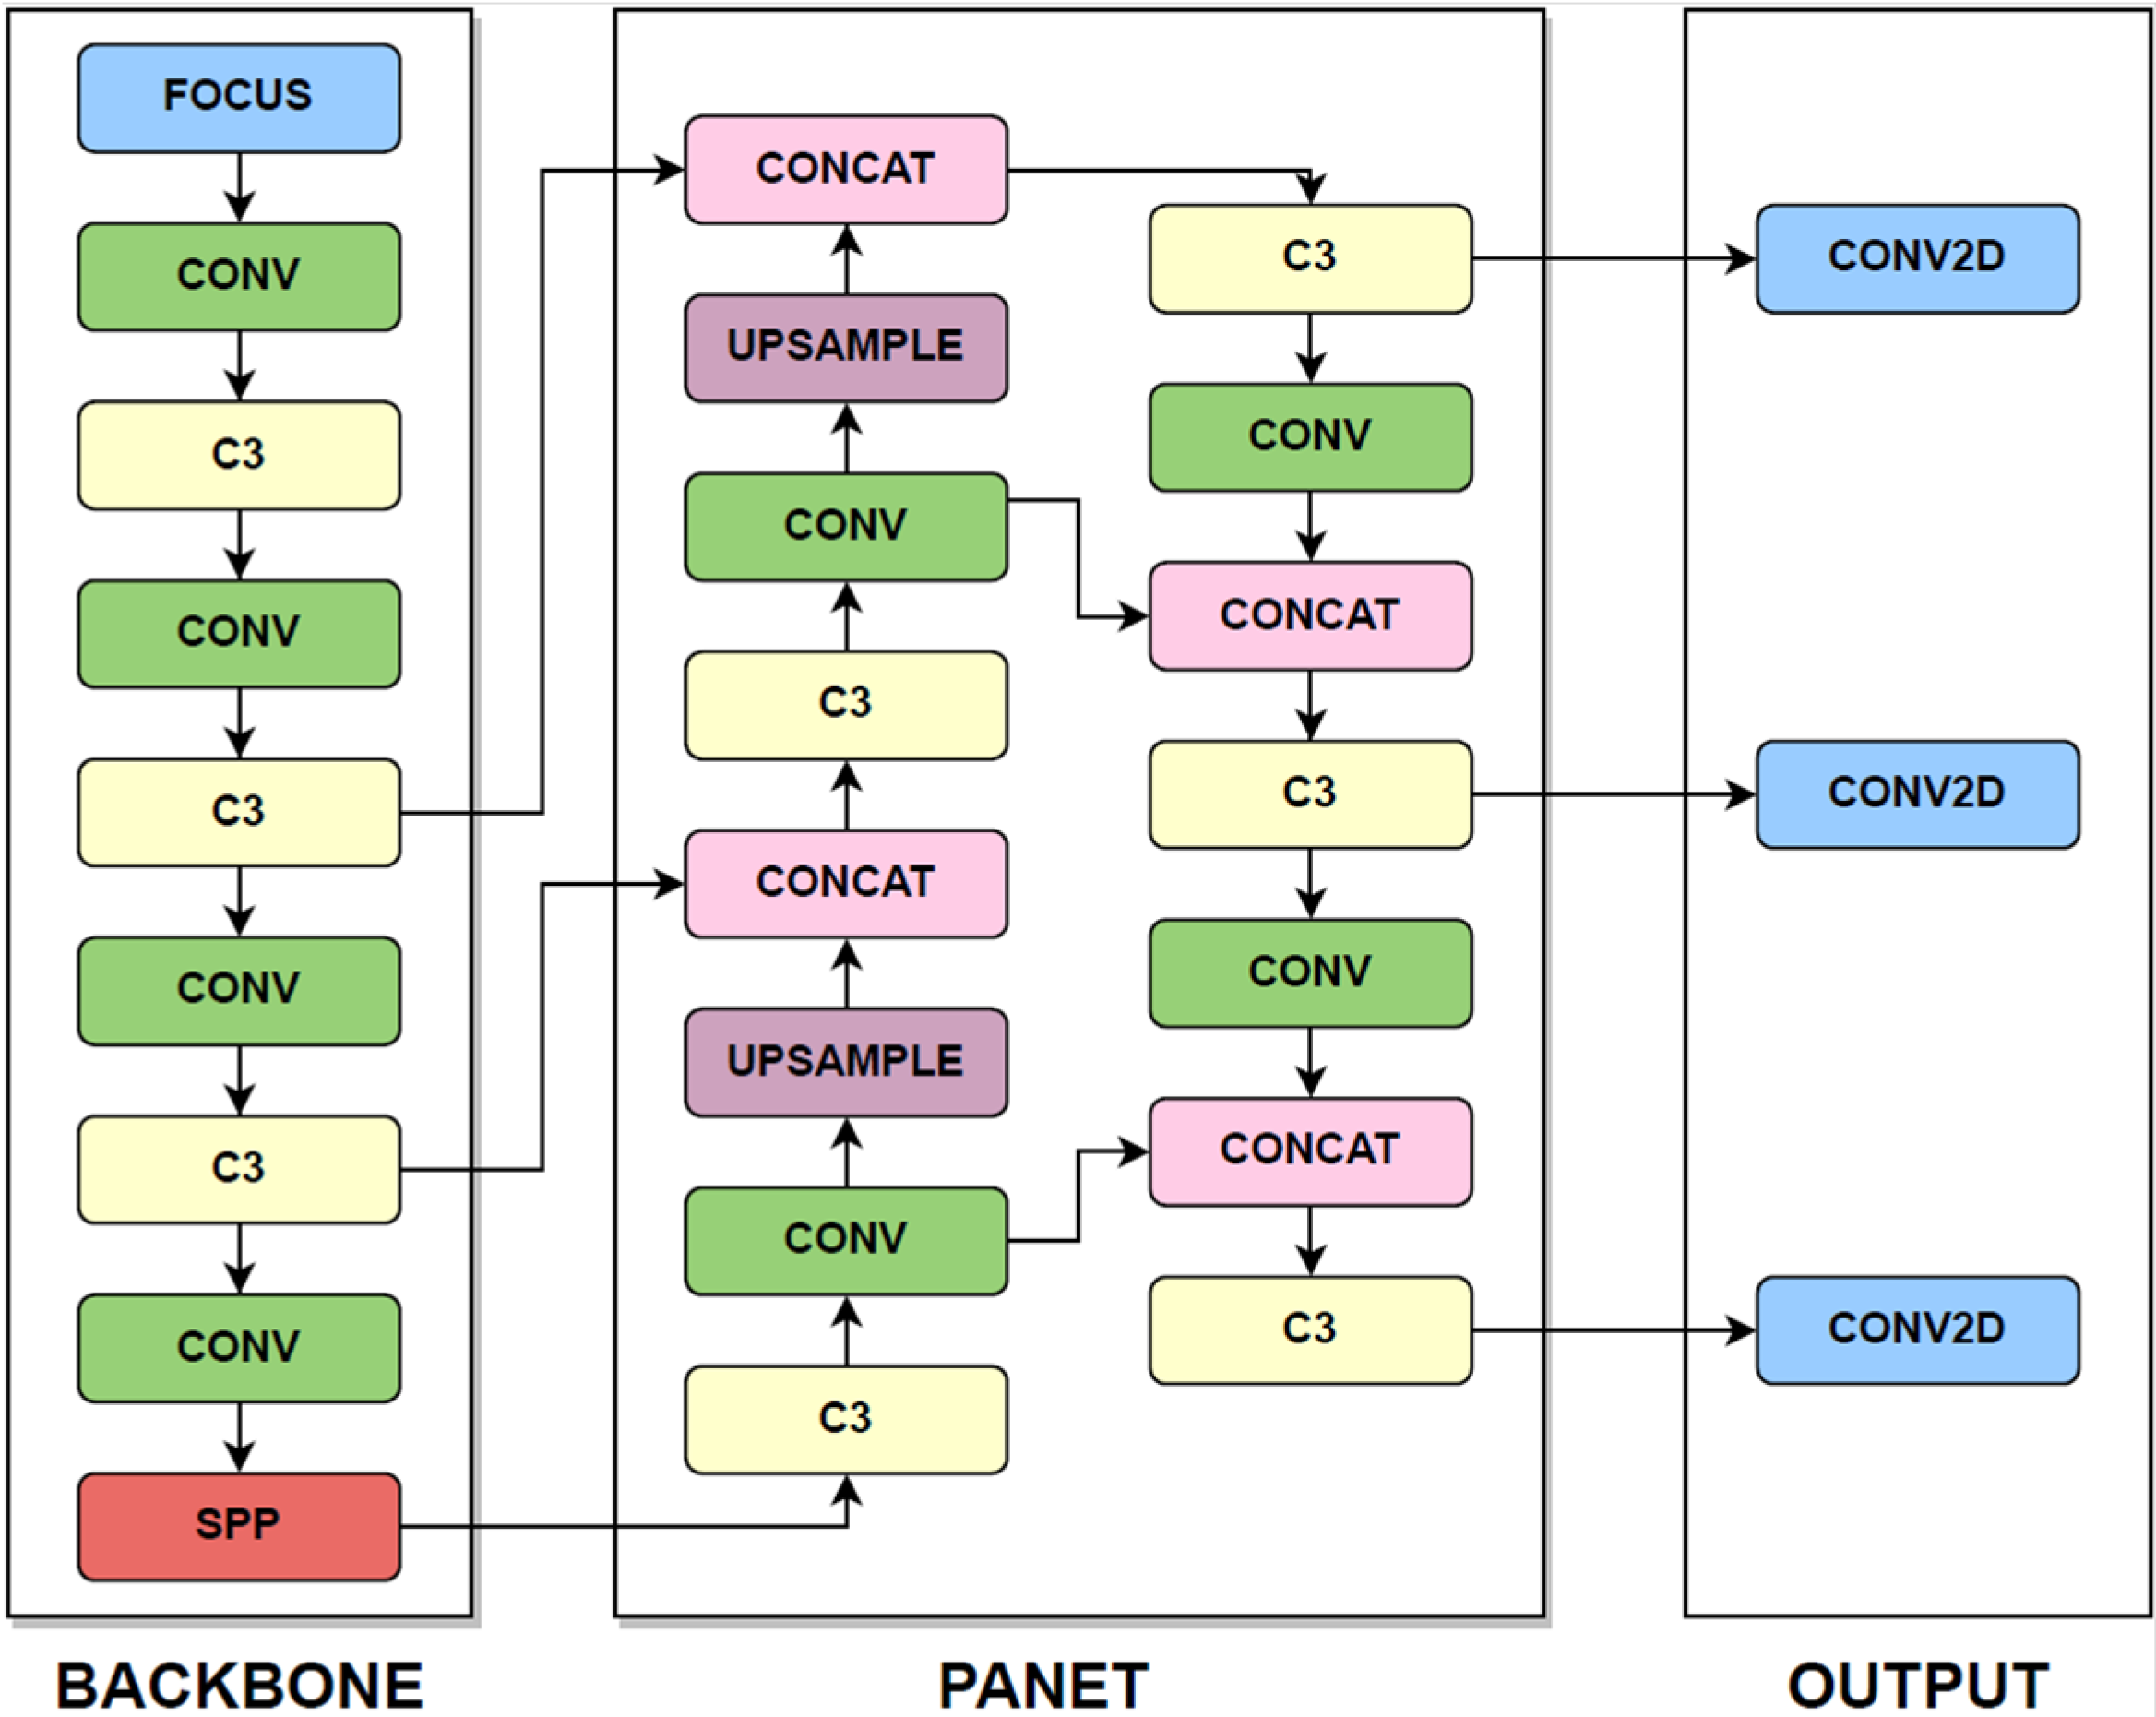
\includegraphics[width=0.65\textwidth]{2/2_teoria/figures/yoloV5.png} % Ajusta el tamaño y ruta
    \caption{Arquitectura de YOLOv5.}
    \label{fig:etiqueta_imagen} % Para referenciar la imagen en el texto
\end{figure}


Finalmente, YOLOv5 es un gran paso adelante en los algoritmos de identificación de objetos, que se aleja de sus predecesores al aprovechar el marco PyTorch e incorporar la red troncal CSPDarknet53 con una nueva arquitectura de agrupación. Esta arquitectura resuelve los problemas de fusión de características y eficiencia computacional, mejorando la precisión de la localización de objetos y reduciendo el tamaño del modelo. La capa de enfoque mejora el uso de la memoria y la eficiencia de propagación.

\subsection{HOG}
El histograma de gradientes orientados (HOG) es un descriptor de características como el detector de bordes de Canny y la transformación de características e invariantes de escala (SIFT). Se utiliza en la visión artificial y el procesamiento de imágenes con el fin de detectar objetos. La técnica cuenta las ocurrencias de orientación de gradiente en la parte localizada de una imagen.

\subsubsection{Prepare la imagen de entrada}
Tome la entrada de la imagen que desea calcular las características HOG. Para ello se tiene que renderizar el tamaño de la imagen a una imagen de 128x64 píxeles (128 píxeles de alto y 64 píxeles de ancho).
\begin{figure}[H]
    \centering
    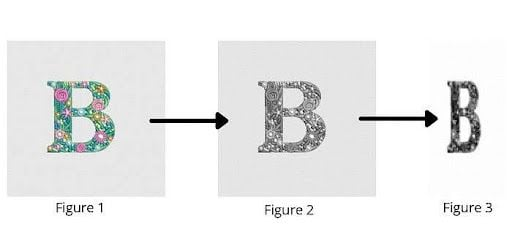
\includegraphics[width=0.60\textwidth]{2/2_teoria/figures/Hog1.jpeg} % Ajusta el tamaño y ruta
    \caption{Preprocesamiento de la imagen.}
    \label{fig:etiqueta_imagen} % Para referenciar la imagen en el texto
\end{figure}

\subsubsection{Calcula el Degradado de la Imagen}
Para calcular el degradado de la imagen debemos conocer que esta compuesto en dos parte gradientes y magnitud.

El gradiente se obtiene combinando la magnitud y el ángulo de la imagen. Considere un bloque de 3x3 píxeles, primero se calcula Gx y Gy para cada píxel utilizando la siguiente fórmula para cada valor de píxel.

\[
G_x(r,c) = I(r,c+1) - I(r,c-1) \quad G_y(r,c) = I(r-1,c) - I(r+1,c)
\]


Después de calcular Gx y Gy, la magnitud y el ángulo de cada píxel se calculan utilizando la fórmula que se menciona a continuación.

\[
\text{Magnitude}(\mu) = \sqrt{G_x^2 + G_y^2} \quad \text{Angle}(\theta) = \left| \tan^{-1}\left(\frac{G_y}{G_x}\right) \right|
\]

\begin{figure}[H]
    \centering
    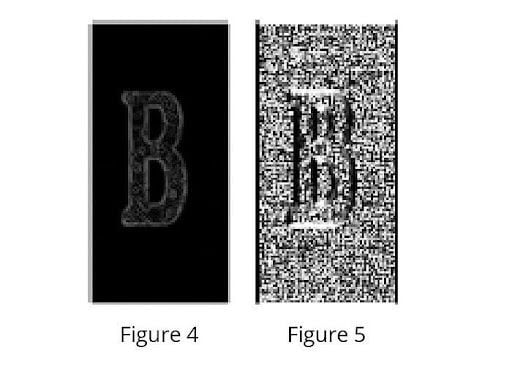
\includegraphics[width=0.55\textwidth]{2/2_teoria/figures/Hog2.jpeg} % Ajusta el tamaño y ruta
    \caption{Degradado de la imagen.}
    \label{fig:etiqueta_imagen} % Para referenciar la imagen en el texto
\end{figure}

\subsubsection{Divide las matrices de degradado para formar un bloque}
Después de obtener el gradiente de cada píxel, las matrices de gradiente (matriz de magnitud y ángulo) se dividen en celdas de 8x8 para formar un bloque. Para cada bloque, se calcula un histograma de nueve puntos. Un histograma de nueve puntos desarrolla un histograma con nueve bins y cada bin tiene un rango de ángulo de 20 grados.
\begin{figure}[H]
    \centering
    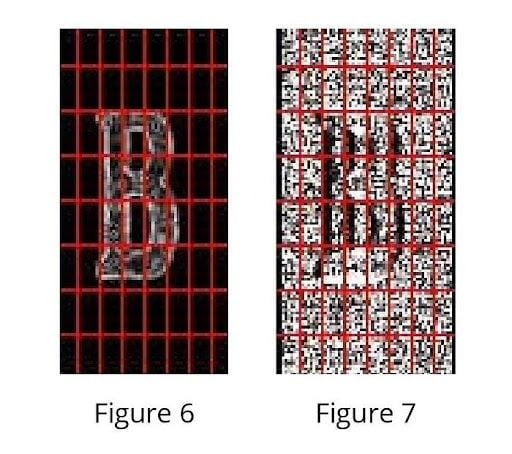
\includegraphics[width=0.55\textwidth]{2/2_teoria/figures/Hog3.jpeg} % Ajusta el tamaño y ruta
    \caption{División de Matrices en bloques.}
    \label{fig:etiqueta_imagen} % Para referenciar la imagen en el texto
\end{figure}

\subsubsection{Agrupar los bloques}
Una vez finalizado el cálculo del histograma para todos los bloques, cuatro bloques de la matriz del histograma de nueve puntos se agrupan para formar un nuevo bloque (2x2). Este aporreado se realiza de forma superpuesta con un paso de ocho píxeles. Para las cuatro celdas de un bloque, concatenamos todos los histogramas de nueve puntos para cada celda constituyente para formar un vector de 36 características.

\begin{figure}[H]
    \centering
    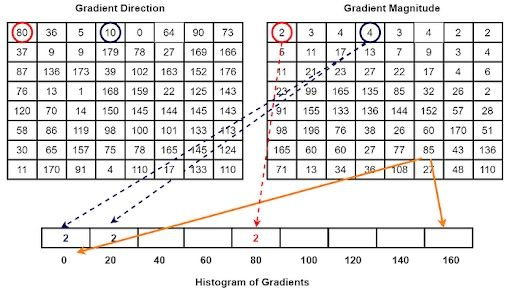
\includegraphics[width=0.50\textwidth]{2/2_teoria/figures/Hog4.jpg} % Ajusta el tamaño y ruta
    \caption{Calculo de Histograma.}
    \label{fig:etiqueta_imagen} % Para referenciar la imagen en el texto
\end{figure}

\subsubsection{Normalizar el valor }
Esta normalización se realiza para reducir el efecto de los cambios en el contraste entre imágenes del mismo objeto. Para normalizar, el valor de k se calcula primero mediante la siguiente fórmula:

\[
k = \sqrt{b_1^2 + b_2^2 + b_3^2 + \dots + b_{36}^2}
\]
\[
f_{bi} = \left[ \left(\frac{b_1}{k}\right), \left(\frac{b_2}{k}\right), \left(\frac{b_3}{k}\right), \dots, \left(\frac{b_{36}}{k}\right) \right]
\]


\subsubsection{Obtenga las características de HOG}
De cada bloque, se recopila un vector de características de 36 puntos. En la dirección horizontal hay 7 bloques y en la dirección vertical hay 15 bloques. Por lo tanto, la longitud total de las características HOG será: 7 x 15 x 36 = 3780. Se obtienen las características HOG de la imagen seleccionada.

\begin{figure}[H]
    \centering
    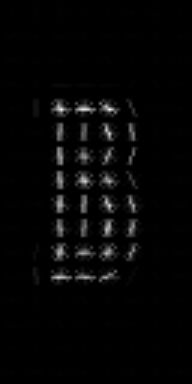
\includegraphics[width=0.20\textwidth]{2/2_teoria/figures/Hog5.jpg} % Ajusta el tamaño y ruta
    \caption{Visualización de características HOG.}
    \label{fig:etiqueta_imagen} % Para referenciar la imagen en el texto
\end{figure}

Por lo tanto, El Histograma de Gradientes Orientados (HoG) se presenta como una técnica robusta y eficiente para la detección de personas, destacándose en entornos dinámicos como las tiendas retail. Su capacidad para identificar siluetas humanas al analizar patrones de gradientes locales lo convierte en una herramienta fundamental para sistemas de vigilancia y análisis de comportamiento del cliente. Esta información permite optimizar la distribución de productos en función del flujo y las preferencias de los consumidores, mejorando la experiencia de compra. Además, HoG no solo es relevante para la detección de personas, sino que también se posiciona como un elemento clave en la transformación digital de las tiendas, conectando la tecnología con la optimización de recursos y la satisfacción del cliente.

% \subsection{SIFT}
% Es un algoritmo para detectar y describir las caracteristicas locales en las imagenes, fue descubierto por David Lowe en 1999. 
% Es un método propuesto por , en el que a una imagen se le transforma en la información en coordenadas invariantes de escala y rotaciones, posteriormente a la luminosidad.

% \subsubsection{Detector}
% Lo primero es obtener un conjunto de puntos de la imagen, los cuales serán denominados keyponints, segun vaya pasando por las diversas etapas, el número de keypoints se irá reduciendo y quedarán los más importantes para ser usados en la comparación.
% \begin{itemize}
%     \item Función scale-space:
%     Se debe realizar una búsqueda de los keypoints en todas las localizaciones de todas las escalas, para lo cual se usa la función continua L(x,y,) convolucionando la imagen I((x,y) y la gausiana.
%     \item Redes Neuronales Convolucionales (CNN): Las CNN destacan por su capacidad para analizar datos visuales, secuenciales y multimodales. En RS, se han utilizado para recomendaciones basadas en texto, imágenes y señales de audio. Ejemplos como DeepCoNN y MusicCNN han mejorado la personalización, mientras que su integración con estructuras de grafos, como CAGCN, aumenta la escalabilidad. Sin embargo, las CNN tienen limitaciones en su capacidad para manejar secuencias largas.
%     \item Redes Neuronales Recurrentes (RNN): Especializadas en datos secuenciales, las RNN han sido fundamentales para recomendaciones basadas en sesiones, como GRU4Rec. Modelos más avanzados, como SASRec, emplean atención para capturar relaciones a largo plazo, y combinaciones con CNN han profundizado en la comprensión de preferencias. A pesar de sus ventajas, enfrentan problemas como gradientes explosivos o desvanecidos, además de un entrenamiento más lento debido a su naturaleza secuencial.
% \end{itemize}


% \subsubsection{Keypoint Descriptor}
% \subsubsection{Matching}

% La coincidencia de imágenes es un aspecto fundamental de muchos problemas de visión artificial, incluido el reconocimiento de objetos o escenas, la resolución de estructuras 3D a partir de múltiples imágenes, la correspondencia estéreo y el seguimiento de movimiento. 
% Se pueden extraer grandes cantidades de características de imágenes típicas con algoritmos eficientes. Además, las características son muy distintivas, lo que permite que una sola característica coincida correctamente con alta probabilidad con una gran base de datos de características, lo que proporciona una base para el reconocimiento de objetos y escenas.
% El reconocimiento de objetos se realiza mediante la coincidencia en primer lugar de cada punto clave de forma independiente de la base de datos de puntos clave extraídos de imágenes de entrenamiento. Muchas de estas coincidencias iniciales serán incorrectas debido a características ambiguas o características que surgen del desorden de fondo. Por lo tanto, primero se identifican las características del grupo al menos 3 que coinciden en un objeto y lo proponen, ya que estos clústeres tienen una probabilidad mucho mayor de ser correctos que las coincidencias de características individuales. A continuación, se comprueba cada clúster realizando un ajuste geométrico detallado al modelo, y el resultado se utiliza para aceptar o rechazar la interpretación.


% El algoritmo SIFT toma una imagen y la transforma en una colección de vectores de características locales. Cada uno de estos vectores de características es distintivo e invariante a cualquier escala, rotación o traslación de la imagen. Estas características no solo son invariantes a la escala y la rotación, sino que también son robustas con respecto al ruido, la oclusión, algunas formas de distorsión afín y los cambios de iluminación. Las características son relativamente fáciles de extraer y también son robustas a la oclusión parcial.

% Por lo tanto, SIFT es un método para extraer características invariantes distintivas de imágenes que se pueden utilizar para realizar una correspondencia confiable entre diferentes imágenes del mismo objeto o escena. El algoritmo SIFT ha llevado a avances significativos en la visión por computadora debido a su eficiencia computacional y efectividad en el reconocimiento de objetos.


\subsection{Datos no Estructurados y Video de Vigilancia}

El análisis de video como fuente de datos no estructurados presenta retos significativos, pero también oportunidades para mejorar la toma de decisiones en el retail. 

Los datos no estructurados no siguen una plantilla específica y predefinida. Además, no están limitados por un modelo de datos específico y predefinido ya que los datos no estructurados no se limitan a documentos de texto sino que abarcan (entre otros) imágenes, grabaciones audiovisuales, correos electrónicos, chats, registros de llamadas, feeds de redes sociales y registros de audio de los centros de llamadas. Los datos no estructurados no se adhieren a los modelos de datos convencionales. Estas formas de datos suelen ser más difíciles de interpretar, según el informe de Deloitte, pero pueden ofrecer una comprensión más completa y holística del panorama general. 

"Debido a que los datos estructurados son más fáciles de trabajar, las empresas ya han podido hacer mucho con ellos", dijo Mikey Shulman. Según algunas estimaciones de la industria, alrededor del 80 por ciento de los datos del mundo no están estructurados.

Es por ello, que los datos no estructurados requiere el uso de técnicas específicas que a menudo son marcadamente diferentes de las empleadas para otros tipos de datos de alta dimensión.

Históricamente, la gestión y utilización de grandes cantidades de datos no estructurados requería mucha mano de obra. Sin embargo, los avances en los modelos de IA han simplificado estas tareas. El contenido de vídeo, en particular, se ha convertido en una importante fuente de datos, ya que ofrece información sobre las reseñas de productos, los comentarios de los clientes y las quejas de las redes sociales.

Por ello, el uso eficaz de los datos no estructurados es esencial para mejorar la participación de los consumidores y aprovechar las diversas fuentes de datos. Ya que, las capacidades de datos no estructurados permiten a los minoristas predecir el comportamiento de los clientes, negociar contratos con proveedores, analizar a la competencia, detectar fraudes y gestionar promociones hiperpersonalizadas. Estas capacidades mejoran los ingresos, el valor del ciclo de vida del cliente y las ganancias a través de la adquisición programática y la gestión de inventario. Por último, los datos no estructurados también son cruciales para recopilar comentarios sobre los productos, informar sobre los ciclos de desarrollo de productos y proporcionar información sobre la demografía de los clientes. Las empresas de bienes de consumo envasados confían en estos datos para comprender el rendimiento del mercado y obtener otros conocimientos valiosos.

\subsection{Sistemas de Recomendación de Distribución de Productos}

Sistema de recomendación son un tipo de sistema de filtrado de información diseñado para predecir y sugerir elementos o contenido, como productos, películas, música o artículos, en los que un usuario podría estar interesado. Estas predicciones se basan en el comportamiento pasado del usuario, sus preferencias o el comportamiento de usuarios similares (\cite{aggarwal2016}). 
El objetivo principal de cualquier sistema de recomendación es mejorar la experiencia del usuario, aumentar el compromiso y facilitar los procesos de toma de decisiones (\cite{berkovsky2008}). Esto es aplicable en varios ámbitos, como el comercio electrónico, el entretenimiento y las redes sociales. Los sistemas de recomendación desempeñan un papel importante tanto en la investigación teórica (académica) como en las aplicaciones prácticas (industria).

En la industria, los sistema de recomendacion mejora la satisfacción del cliente e impulsa el crecimiento de los ingresos al proporcionar sugerencias personalizadas (\cite{amatriain2016}). Grandes corporaciones como Amazon, Netflix y Spotify integran RS en sus operaciones, contribuyendo significativamente a sus modelos de negocio. Por ejemplo, Amazon informa que el 35\% de sus ingresos proviene de su RS (\cite{mackenzie2013}), mientras que Netflix atribuye ingresos de aproximadamente \$ 33.7 mil millones y su éxito en la retención de clientes significativamente a su RS (\cite{iqbal2024}). Se prevé que el mercado mundial de motores de recomendación, según Precision Reports [12] (\cite{precision2024}), experimente un crecimiento sustancial entre 2023 y 2030, lo que pone de manifiesto su creciente importancia en las estrategias empresariales. Los algoritmos que preservan la privacidad y la mitigación de sesgos también se están convirtiendo en áreas clave de enfoque para los profesionales de la industria.

La investigación o las aplicaciones centradas en la práctica suelen considerar las RS como herramientas esenciales para mejorar la participación de los usuarios, la retención y el crecimiento empresarial (\cite{amatriain2016, melville2010}). Es necesaria la colaboración entre el mundo académico y la industria para abordar tanto los desafíos técnicos como las demandas del mundo real, lo que a su vez mejora la satisfacción del usuario y el valor empresarial. Esta interdependencia pone de relieve la creciente importancia de esas asociaciones.

La importancia del sistema de recomendación ha crecido exponencialmente frente a los grandes datos y los avances en la inteligencia artificial (\cite{adomavicius2005, ricci2022}). A medida que los usuarios interactúan con las plataformas digitales, generan grandes cantidades de datos que pueden aprovecharse para hacer precisos



\subsubsection{Deep Learning en los Sistemas de Recomendación}
En los últimos años, el deep learning se ha consolidado como un estándar en los sistemas de recomendación (RS). Esta evolución ha permitido abordar desafíos complejos, mejorando la precisión y personalización de las recomendaciones gracias a diversas arquitecturas de redes neuronales profundas.

\begin{itemize}
    \item Redes Perceptronas Multicapa (MLP): Tradicionalmente, los RS utilizaban métodos lineales como la factorización matricial, que son limitados para capturar interacciones complejas entre usuarios y elementos. Las MLP, mediante múltiples capas profundas, modelan estas relaciones no lineales, logrando mayor precisión. Sin embargo, presentan desafíos como la complejidad, el riesgo de sobreajuste y problemas de interpretabilidad.
    \item Redes Neuronales Convolucionales (CNN): Las CNN destacan por su capacidad para analizar datos visuales, secuenciales y multimodales. En RS, se han utilizado para recomendaciones basadas en texto, imágenes y señales de audio. Ejemplos como DeepCoNN y MusicCNN han mejorado la personalización, mientras que su integración con estructuras de grafos, como CAGCN, aumenta la escalabilidad. Sin embargo, las CNN tienen limitaciones en su capacidad para manejar secuencias largas.
    \item Redes Neuronales Recurrentes (RNN): Especializadas en datos secuenciales, las RNN han sido fundamentales para recomendaciones basadas en sesiones, como GRU4Rec. Modelos más avanzados, como SASRec, emplean atención para capturar relaciones a largo plazo, y combinaciones con CNN han profundizado en la comprensión de preferencias. A pesar de sus ventajas, enfrentan problemas como gradientes explosivos o desvanecidos, además de un entrenamiento más lento debido a su naturaleza secuencial.
\end{itemize}


El deep learning ha revolucionado los sistemas de recomendación, permitiendo una mejor personalización, escalabilidad y precisión. Sin embargo, enfrenta retos como la complejidad computacional, la interpretabilidad y el manejo de datos secuenciales o ruidosos. La evolución continua de estas tecnologías promete desarrollar sistemas más avanzados y adaptables, beneficiando aún más a diversas industrias como el comercio, entretenimiento y noticias.

% \subsection{Optimización de Flujo de Cliente de un Retail}
% La opotimización de flujo de cliente son combinaciones de estrategias para mejorar la experiencia del cliente generando una experiencia de compra fluida y agradable ya que los productos estan a disposición del cliente evitando aglomeración. Ademas de tener un espacio funcional donde los clientes circulen sin sentirse apretados contribuyendo al ambiente general del retail.
% Las tecnologías de visión por computadora han permitido a los minoristas realizar análisis detallados del movimiento y comportamiento de los clientes, lo cual es esencial para gestionar el flujo de manera efectiva (Labeller et al., 2020; Yenra, 2020).

% La implementación de cámaras de vigilancia inteligentes permite monitorear en tiempo real el tráfico en diferentes áreas de la tienda y, a través de algoritmos de visión por computadora, generar mapas de calor que muestran las zonas de mayor actividad. Estos mapas ayudan a identificar los "puntos calientes" y los "puntos fríos" de la tienda, lo cual proporciona datos críticos para reubicar productos en áreas estratégicas y asegurar que las áreas de alto interés tengan suficiente espacio para el tráfico de clientes (Yenra, 2020). Según Labeller et al. (2020), este tipo de datos es crucial para ajustar la disposición de productos y organizar el diseño del espacio comercial de forma que guíe de manera natural el flujo de personas, evitando las aglomeraciones y optimizando el tiempo que los clientes pasan en cada área.

% \subsection{Métricas de Comportamiento en un Retail}
% La aplicación de visión por computadora y técnicas de inteligencia artificial en el ámbito del retail ha facilitado el análisis de patrones de comportamiento de clientes mediante cámaras de vigilancia y mapas de calor. Estos sistemas de análisis visual permiten detectar áreas de alta afluencia dentro de la tienda, lo que resulta crucial para mejorar la disposición de productos y maximizar el tiempo que los clientes permanecen en las áreas de interés. Los mapas de calor generados muestran las zonas de mayor y menor actividad, proporcionando datos que los minoristas pueden usar para ajustar estrategias de marketing y optimización del diseño de la tienda (Almeida et al., 2020; Lee et al., 2022).

% \subsection{Eficiencia Operativa de un Retail}
% La eficiencia operativa en el sector retail se refiere a la capacidad de optimizar sus recursos, procesos y tiempo de manera que maximice la rentabilidad y el servicio al cliente, minimizando los costos.
% Los sistemas de visión por computadora permiten monitorear el inventario en tiempo real, detectar rápidamente cuándo los productos necesitan reposición y reducir el tiempo de inactividad en la tienda. De acuerdo con Yenra (2020), estos sistemas automatizan tareas como la verificación de inventarios y las alertas de reposición, permitiendo que el personal se enfoque en actividades más estratégicas y de atención directa al cliente. Esta automatización contribuye a reducir costos operativos asociados con la gestión manual de inventarios y disminuye la frecuencia de situaciones de "producto agotado", lo cual es clave para mantener altos niveles de satisfacción del cliente.





 

\section{Marco Conceptual}
\subsection{Visión por Computadora}
La visión artificial es un campo de la inteligencia artificial (IA) que utiliza el aprendizaje automático y las redes neuronales para enseñar a los ordenadores y sistemas a obtener información significativa de imágenes digitales, vídeos y otros elementos visuales, y a hacer recomendaciones o tomar medidas cuando ven defectos o problemas (\cite{IBM2023vision}).

\subsection{Sistemas de Recomendación}
Los sistemas de recomendación (RS) son una de las soluciones que ayudan a los usuarios a gestionar la sobrecarga de opciones. Las RS son herramientas importantes que permiten a las personas tomar decisiones alineadas con sus necesidades y preferencias (\cite{Amin2020}).

\subsection{Datos No Estructurados}
Los datos no estructurados se definen comúnmente como datos que no están disponibles en formatos estructurados predefinidos, como los formatos tabulares. En la literatura, los datos digitales no estructurados a menudo se denominan indistintamente "big data", "datos digitales", "datos textuales no estructurados" y se describen como "de alta dimensión", "gran escala", "ricos", "multivariados" o "sin procesar" (\cite{sarmiento2023challenges}).


\subsection{YOLO}
Segun (\cite{Redmon2016YOLO}) You Only Look Once (YOLO), es un enfoque innovador que trata sobre examinar las imagenes para detectar objetos y posiciones. Además, en el paradigma YOLO, emplea una sola red neuronal convolucional para predecir cuadros delimitadores y las probabilidades de clase para una imagen completa (\cite{Hussain2023YOLO}).


\subsection{Inteligencia Artificial Aplicada a Retail}
La inteligencia artificial (IA) se refiere a la simulación de procesos de inteligencia humana por parte de máquinas, ejecutadas principalmente a través de sistemas informáticos. Además, segun (\cite{Cocco2022}) La inteligencia artificial (IA) se refiere al desarrollo de sistemas informáticos capaces de realizar tareas que normalmente requieren inteligencia humana, como el aprendizaje, el razonamiento y la toma de decisiones


\subsection{HOG (Histogram of Oriented Gradients)}
Histogram of oriented grafients es HOG es un tipo de “descriptor de características”. El objetivo de un descriptor de características es generalizar el objeto de tal forma que el mismo objeto. (\citet{pardoHOG}). Los descriptores HOG son descriptores utilizados para la detección de objetos, los cuales están basados en histogramas de gradientes orientados (\citep{avilaHOG}).

\subsection{SIFT (Scale-Invariant Feature Transform)}

Segun (\cite{AlegreFernandez2018}) Scale invariant feature transform es un método que permite detectar puntos característicos en una imagen y luego describirlos mediante un histograma orientado de gradientes. Ademas es el reconocimiento de objetos, y especialmente cuando hay oclusión o el fondo está lleno de objetos desordenados (clutter).



\section{Hipótesis}
\subsection{Hipótesis General}
HG: \newcommand{\HipotesisGeneral}{
Mediante la implementación de un sistema de visión por computadora se logrará recomendar una mejor distribución de productos para optimizar el flujo de clientes y aumentar la eficiencia operativa en tiendas retail en el 2024.
}
\HipotesisGeneral


\subsection{Hipótesis Específicas}
\newcommand{\Hone}{
La identificacion del mejor enfoque permite la detección y ratreo de personas en tiempo real y con, alta precisión.
}
\newcommand{\Htwo}{
La utilización de los indicadores de movimiento y permanencia de los clientes ayudará a identificar zonas altas y baja afluencia en la tienda.
}
\newcommand{\Hthree}{
Definiendo una arquitectura que procese video generará recomendaciones rápidas y precisas.
}
\newcommand{\Hfour}{
La implementación de un sistema de gestión de inventarios en tiempo real reducirá los tiempos de espera de los clientes y aumentará la satisfacción del cliente.
}

\begin{itemize}
	\item HE1: {\Hone}
	\item HE2: {\Htwo}
	\item HE3: {\Hthree}
	\item HE4: {\Hfour}
\end{itemize}

\chapter{METODOLOGÍA DE LA INVESTIGACIÓN}
\section{Diseño de la investigación}
En el presente capítulo se define el diseño, tipo y enfoque de la investigación. Asimismo, se explica la población y muestra, es decir la base de dato que va a ser usada. Finalmente, se explican las técnicas usadas para la recolección de datos, el preprocesamiento de los mismos y el modelo Deep Learning para la creación del modelo de clasificación.
\subsection{Diseño experimental}
El diseño de la presente investigación es de tipo cuasi-experimental, ya que no se puede realizar una asignación aleatoria de los sujetos en el entorno de tienda retail. Se implementará un sistema de recomendación en el cual se utilizará el modelo de visión por computadora YOLO (You Only Look Once) para la detección y seguimiento de clientes en la tienda. A partir de los datos recopilados, se generará un mapa de calor que permita identificar las áreas de mayor y menor flujo de clientes. Este mapa de calor servirá como insumo para el sistema de recomendación de redistribución de productos en los anaqueles, buscando optimizar el flujo de clientes y lograr una distribución más uniforme en la tienda. El sistema ajustará la disposición de los productos para balancear el tráfico en el espacio de tienda y mejorar la experiencia de compra.

\subsection{Tipo explicativo}
El nivel del trabajo de investigación es explicativo, debido a que el diseño de un sistema de visión por computadora para el sistema de recomendación en el sector retail busca comprender la relación causa efecto entre la implementación del sistema y los resultados obtenidos, es decir como las recomendaciones generadas por el sistema basado en visión por computadora afectan la disposición de los productos, las ventas y la experiencia del cliente. Este enfoque es coherente con lo descrito por Sampieri et al. (2014), quienes señalan que el nivel explicativo busca identificar las causas de un fenómeno y sus efectos, aportando comprensión sobre las condiciones que determinan su ocurrencia.

\subsection{Enfoque cuantitativo}
El enfoque de la investigación es cuantitativo, debido a que se utilizan instrumentos para la identificación y medición del objeto de estudio el cual es el sistema de recomendación para el sector retail a través del recorrido de los clientes, se utilizaran la técnica de visión por computadora (YOLO) cuyos resultado numéricos servirán como el tiempo de permanencia de los clientes en la tienda para el mapa de calor por zonas, la precisión del modelo como la precisión, recall, F1-score y tiempo del procesamiento, serán analizados. Según Sampieri, Fernández y Baptista (2014), la investigación cuantitativa permite medir fenómenos y realizar análisis estadísticos para generalizar resultados, lo que asegura la objetividad en la interpretación de los datos obtenidos.

\section{Población y muestra}

\begin{table}[H]
\centering

\begin{tabular}{|>{\raggedright}p{3.5cm}|p{10cm}|}
\hline
\textbf{Población} & La población de esta investigación está compuesta por tiendas retail pequeñas y medianas que cuentan con cámaras de vigilancia en diversas regiones del Perú. Estas tiendas utilizan sistemas de grabación para aplicar técnicas de visión por computadora como YOLO, optimizando la distribución de productos y mejorando la experiencia del cliente. \\ \hline
\textbf{Muestra}   & 50 videos de videovigilancia corresponde al minimarket “La Económica”, ubicado en Puquio, provincia de Lucanas, Ayacucho, Perú. Este minimarket cuenta videos que captura videos del comportamiento de los clientes en distintas zonas del establecimiento. Los datos obtenidos se utilizarán para aplicar el método YOLO y generar recomendaciones sobre la redistribución de productos en bloques de zonas. El muestreo es no probabilístico por conveniencia, dado el acceso a datos relevantes. \\ \hline
\textbf{Unidad de Análisis}  & Cada video de vigilancia capturado será una unidad de análisis, de la cual se extraerán métricas clave como la distribución del tiempo de permanencia de los clientes en diferentes zonas de la tienda. \\ \hline
\textbf{Variables y Tipos de Variables}  & Las variables analizadas serán cuantitativas y continuas, centradas en datos numéricos como el tiempo de permanencia, la precisión del modelo y otras métricas de rendimiento. \\ \hline
\end{tabular}
\caption{Tabla de Población y la Muestra}
\label{tab:poblacion_muestra}
\end{table}


\section{Operacionalización de Variables}

\begin{table}[H]
\centering
\begin{tabular}{|>{\raggedright}p{3.5cm}|p{5cm}|p{5.5cm}|}
\hline
\textbf{VARIABLE Y DEFINICIÓN} & \textbf{INDICADOR} & \textbf{FÓRMULA} \\ \hline

\textbf{Sistema de Recomendacion de Productos.}
%Generación de sugerencias para mejorar la distribución de productos en función del análisis de los videos.
& Efectividad de las recomendaciones & $\frac{\text{Incremento de ventas post-recomendación}}{\text{Ventas previas}}$  \\ \cline{2-3}&Aumento en tiempo de permanencia en zonas recomendadas & 
$\frac{\text{Tiempo en zonas recomendadas}}{\text{Tiempo total en la tienda}}$ \\ \hline

\textbf{Visión por Computadora} & Resolución del video. & Cantidad de pixeles encontrados en el video \\ \cline{2-3} & Procesamiento del video & Nivel de nitidez, contraste o ruido encontrado en la imagen\\ \hline
 
\textbf{Modelo de Clasificación} & Accuracy & $\frac{TP + TN}{TP + FP + FN + TN}$ \\ \cline{2-3} 
& Precisión & $\frac{TP}{TP + FP}$ \\ \cline{2-3} 
& Recall & $\frac{TP}{TP + FN}$ \\ \cline{2-3} 
& F1 & $2 \cdot \frac{\text{Precisión} \cdot \text{Recall}}{\text{Precisión} + \text{Recall}}$ \\ \hline
% & ROC AUC & $P(\text{score}(x^+) > \text{score}(x^-))$ \\ \hline
\end{tabular}
\caption{Definición de variables}
\label{tab:definicion_variables}
\end{table}

Donde:
\begin{itemize}
    \item TP: Verdaderos Positivos.
    \item FP: Falsos Positivos.
    \item TN: Verdaderos Negativos.
    \item FN: Falsos Negativos.
\end{itemize}


\section{Técnicas de recolección de datos}

En esta sección se describen las técnicas empleadas para la recolección de datos visuales y demográficos, los cuales son esenciales para desarrollar el sistema de visión por computadora propuesto.

\subsection{Configuración Inicial}

Para la recolección de datos se instalaron cámaras de visión estándar en ``La Económica''. Se definieron tres áreas de interés: zona de entrada, pasillo central y área de cajas. Estas áreas se eligieron en base al flujo promedio de clientes observado.

\subsection{Procedimientos de Recolección}

\begin{table}[H]
\centering
\caption{Actividades para la recolección de datos}
\label{table:recoleccion}
\begin{tabular}{|p{5cm}|p{10cm}|}
\hline
\textbf{Actividad} & \textbf{Descripción} \\ \hline
\textbf{Grabación inicial} & Las cámaras capturaron datos en intervalos de 15 fps durante las horas pico (10:00 a 13:00 y 17:00 a 20:00) por un periodo de 14 días. \\ \hline
\textbf{Segmentación de video} & Se segmentaron los videos en intervalos de 10 segundos para analizar patrones individuales de clientes. \\ \hline
\textbf{Etiquetado manual} & Un equipo de 3 personas etiquetó manualmente las zonas transitadas utilizando software especializado como LabelImg. \\ \hline
\textbf{Validación de datos} & Los datos etiquetados fueron validados por un especialista en análisis de comportamiento en tiendas retail. \\ \hline
\end{tabular}
\end{table}

\subsection{Instrumentos Utilizados}

\begin{itemize}
    \item \textbf{Cámaras de visión estándar:} Configuradas con resolución 1080p y un ángulo de visión de 90 grados.
    \item \textbf{Software de etiquetado:} LabelImg para crear conjuntos de datos anotados que incluyan información como zonas de alto y bajo tránsito.
    
\end{itemize}

\textbf{Entregables:} Conjunto de datos etiquetados con información de flujo de clientes y zonas transitadas.

\subsection{Precisión en la Recolección de Datos}

Para garantizar la calidad de los datos recolectados, se calcularon métricas de confiabilidad:

\begin{equation}
\text{Precisión en etiquetado} = \frac{\text{Etiquetas correctas validadas}}{\text{Total de etiquetas generadas}} \times 100
\end{equation}

\begin{equation}
\text{Cobertura de cámaras} = \frac{\text{Área cubierta por cámaras}}{\text{Área total de la tienda}} \times 100
\end{equation}

\textbf{Resultados esperados:}
- Cobertura del 85\% de las áreas clave de la tienda.
- Precisión del 90\% en el etiquetado manual de los datos recolectados.

% Nisi porta lorem mollis aliquam ut porttitor leo. Aenean pharetra magna ac placerat vestibulum. Est placerat in egestas erat imperdiet sed euismod. Velit euismod in pellentesque massa placerat. Enim praesent elementum facilisis leo vel fringilla. Ante in nibh mauris cursus mattis molestie a iaculis. Erat pellentesque adipiscing commodo elit at imperdiet dui accumsan sit. Porttitor lacus luctus accumsan tortor posuere ac ut. Tortor at auctor urna nunc id. A iaculis at erat pellentesque adipiscing commodo elit.

% \LaTeX{} is great at typesetting mathematics. Let $X_1, X_2, \ldots, X_n$ be a sequence of independent and identically distributed random variables with
% \begin{equation}
% 	S_n = \frac{X_1 + X_2 + \cdots + X_n}{n}
% 	= \frac{1}{n}\sum_{i}^{n} X_i
% 	\label{eq1}
% \end{equation}

% La Ecuación \ref{eq1} denote their mean. Then as $n$ approaches infinity, the random variables $$\sqrt{n}(S_n - \mu)$$ converge in distribution to a normal $\mathcal{N}(0, \sigma^2)$.

\section{Técnicas para el Procesamiento y Análisis de la Información}

\subsection{Metodología de Implementación de la Solución}

Según Szeliski (2010), las etapas fundamentales en un sistema de visión por computadora incluyen la adquisición, preprocesamiento, extracción de características, y modelado. En este proyecto, estas etapas han sido adaptadas para resolver el problema de optimización en la distribución de productos en tiendas retail, como se detalla a continuación.
\begin{figure}[H]
    \centering
    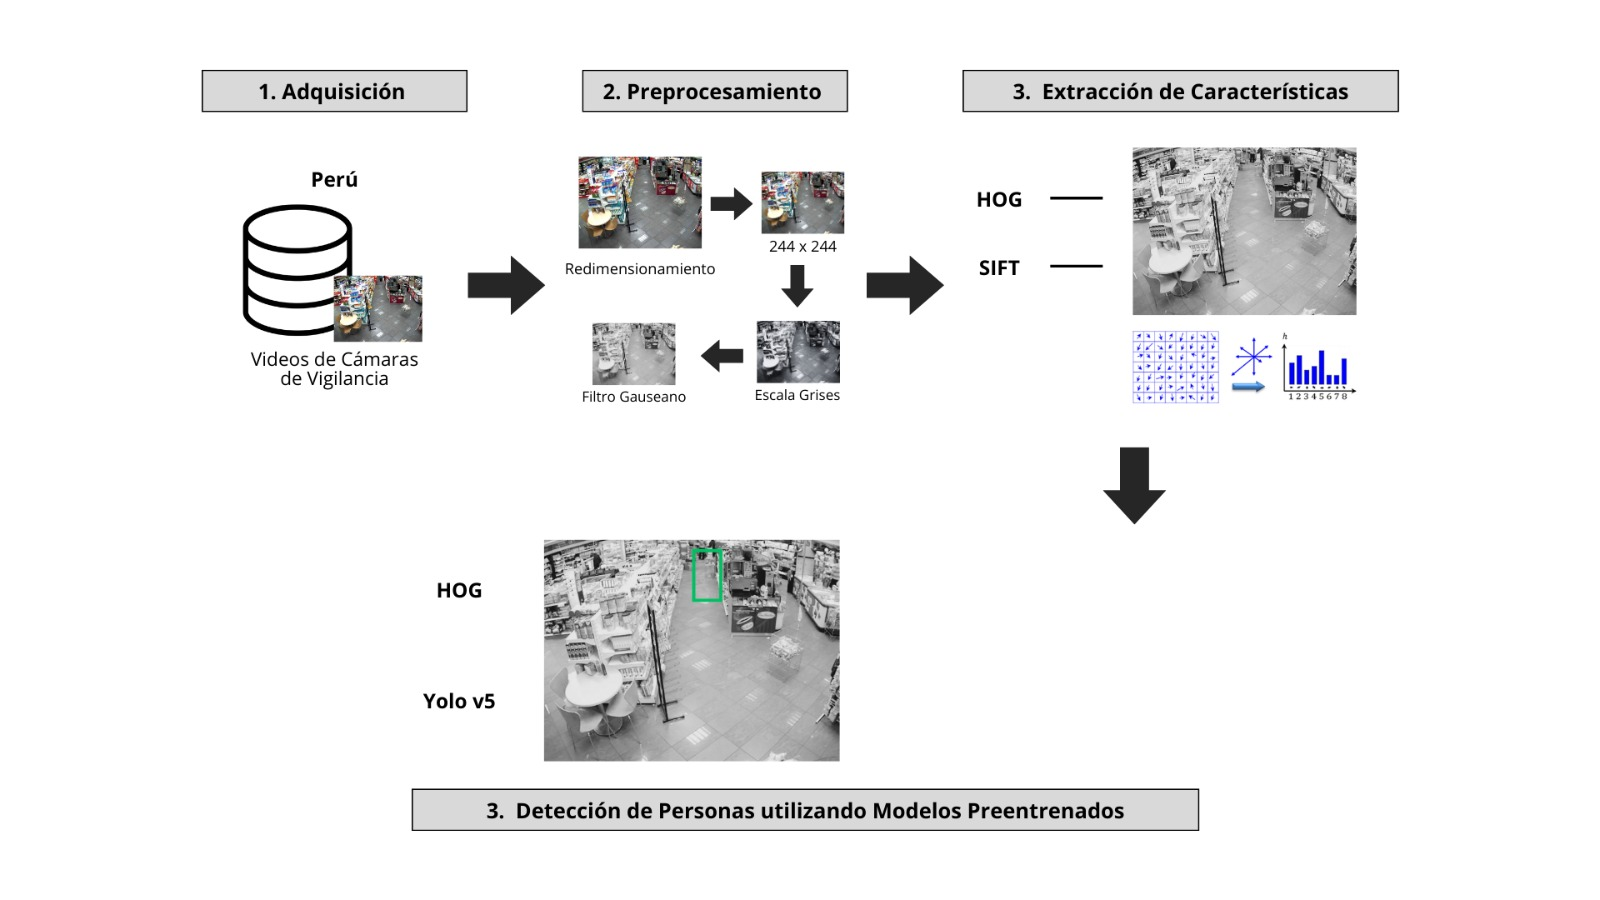
\includegraphics[width=0.8\textwidth]{3/figures/metodologia1.jpg} % Ajusta el tamaño y ruta
    \caption{Metodología}
    \label{fig:etiqueta_imagen} % Para referenciar la imagen en el texto
\end{figure}
\subsubsection{Adquisición}

La adquisición de datos fue realizada mediante la instalación de cámaras de visión estándar en el negocio retail ``La Económica'', recopilando imágenes de las áreas de interés clave. Estas cámaras se configuraron para registrar imágenes de 1080p con una frecuencia de 15 fps.

\begin{table}[H]
\centering
\caption{Actividades etapa de adquisición}
\label{table:adquisicion}
\begin{tabular}{|p{5cm}|p{8cm}|}
\hline
\textbf{Actividades} & \textbf{Descripción} \\ \hline
Identificación de áreas clave & Selección de zonas con alta densidad de tránsito de clientes. \\ \hline
Configuración de cámaras & Instalación y calibración de cámaras para capturar datos relevantes. \\ \hline
Grabación inicial & Grabación continua durante horarios pico por un periodo de 14 días. \\ \hline
\end{tabular}
\end{table}

\textbf{Entregables:} Datos en formato de video y frames estáticos clasificados por ubicación y rango horario.

\subsubsection{Preprocesamiento}

El preprocesamiento consistió en la normalización y mejora de las imágenes adquiridas. Se utilizaron técnicas como:

\begin{itemize}
    \item \textbf{Redimensionamiento:} Ajuste de las imágenes a $224 \times 224$ píxeles para compatibilidad con modelos.
    \item \textbf{Conversión a escala de grises:} Reducción de la dimensionalidad de los datos.
    \item \textbf{Eliminación de ruido:} Aplicación de filtros de mediana y gaussiano.
    \item \textbf{Data augmentation:} Incremento de la diversidad mediante rotaciones, traslaciones y ajustes de brillo.
\end{itemize}

\begin{equation}
I'(x, y) = \frac{I(x, y) - \text{min}(I)}{\text{max}(I) - \text{min}(I)} \times 255
\label{eq:normalization}
\end{equation}

\subsubsection{Extracción de Características}

Se implementaron técnicas avanzadas de extracción de características para identificar patrones relevantes en las imágenes:

\begin{table}[H]
\centering
\caption{Técnicas de extracción de características utilizadas}
\label{table:features}
\begin{tabular}{|l|p{10cm}|}
\hline
\textbf{Técnica} & \textbf{Descripción} \\ \hline
HOG (Histogram of Oriented Gradients) & Permite detectar bordes y gradientes locales. \\ \hline
SIFT (Scale-Invariant Feature Transform) & Detecta puntos de interés robustos a escala y rotación. \\ \hline
\end{tabular}
\end{table}

\subsubsection{Detección de Personas utilizando Modelos Preentrenados}

En esta etapa del proceso, la detección de personas se lleva a cabo mediante el uso de modelos ya entrenados, aprovechando arquitecturas probadas y reconocidas en el estado del arte, específicamente \textbf{HOG} (Histogram of Oriented Gradients), \textbf{SIFT} (Scale-Invariant Feature Transform) y \textbf{YOLOv5} (You Only Look Once, versión 5). Estas técnicas permiten identificar y localizar a las personas dentro de las imágenes sin necesidad de desarrollar un modelo propio mediante entrenamiento, validación o prueba. 

\paragraph{Detección con HOG.} El modelo de \textit{Histogram of Oriented Gradients (HOG)}, preentrenado para la detección de personas, se utiliza para extraer características visuales basadas en gradientes locales. El HOG genera un descriptor robusto que facilita la identificación de formas humanas, incluso en condiciones de iluminación variables. Este modelo preentrenado permite una detección confiable al aplicar directamente su clasificador lineal sobre las características calculadas.

\paragraph{Detección con SIFT.} La técnica \textit{Scale-Invariant Feature Transform (SIFT)} es empleada para identificar puntos de interés clave en las imágenes. Aunque SIFT no está específicamente diseñado para la detección de personas, su integración como un método de extracción de características complementa los resultados de HOG al detectar patrones invariantes a escala y rotación que están presentes en las siluetas humanas.

\paragraph{Detección con YOLOv5.} \textit{You Only Look Once, versión 5 (YOLOv5)} es un modelo preentrenado para la detección en tiempo real de personas. Este modelo, ampliamente optimizado y eficaz, permite localizar objetos específicos (en este caso, personas) mediante bounding boxes en las imágenes. Gracias a su enfoque basado en regresión, YOLOv5 identifica simultáneamente la clase del objeto y sus coordenadas espaciales. Al ser una solución preentrenada, su implementación se limita a la inferencia, sin necesidad de ajustes adicionales.

\paragraph{Implementación General.} La integración de estos modelos se realiza con herramientas preexistentes y bien documentadas, como bibliotecas de Python (\textit{OpenCV, TensorFlow, PyTorch}). A través de ellas, las imágenes del dataset se procesan directamente para obtener las detecciones de personas, siguiendo el flujo definido en la metodología. Este enfoque elimina la necesidad de separar el dataset en subconjuntos de entrenamiento, validación y prueba, dado que los modelos preentrenados ya contienen la información requerida para la detección eficiente.

\begin{figure}[H]
    \centering
    \includegraphics[width=0.8\textwidth]{ruta_a_diagrama}
    \caption{Flujo de detección de personas utilizando modelos preentrenados (HOG, SIFT y YOLOv5).}
    \label{fig:deteccion_personas}
\end{figure}

Este esquema metodológico asegura una detección precisa y eficiente de personas, empleando herramientas consolidadas y reduciendo la carga computacional asociada al entrenamiento de modelos desde cero.


\section{Medición de Resultados}

Para evaluar el desempeño del sistema, se utilizaron las métricas estándar de clasificación:

\begin{equation}
\text{Accuracy} = \frac{TP + TN}{TP + TN + FP + FN}
\end{equation}

\begin{equation}
\text{Precision} = \frac{TP}{TP + FP}, \quad \text{Recall} = \frac{TP}{TP + FN}
\end{equation}

Donde:
\begin{itemize}
    \item TP: Verdaderos Positivos.
    \item FP: Falsos Positivos.
    \item TN: Verdaderos Negativos.
    \item FN: Falsos Negativos.
\end{itemize}

\section{Cronograma de Actividades}

El cronograma se desarrolló considerando las fases principales del proyecto, distribuidas a lo largo de 9 meses.

\begin{table}[H]
\centering
\caption{Cronograma de actividades}
\label{table:cronograma}
\begin{tabular}{|p{4cm}|p{8cm}|}
\hline
\textbf{Fase} & \textbf{Meses y Actividades} \\ \hline
Adquisición de datos & Enero - Febrero: Configuración de cámaras y recolección inicial de imágenes. \\ \hline
Preprocesamiento & Marzo - Abril: Limpieza y normalización de datos. \\ \hline
Entrenamiento y Validación & Mayo - Julio: Entrenamiento de modelos y validación de resultados. \\ \hline
Evaluación y Documentación & Agosto - Septiembre: Evaluación del sistema, generación de conclusiones y recomendaciones. \\ \hline
\end{tabular}
\end{table}

\section{Presupuesto}

\begin{table}[H]
\centering
\caption{Presupuesto estimado del proyecto}
\label{table:presupuesto}
\begin{tabular}{|l|p{7cm}|r|}
\hline
\textbf{Recurso} & \textbf{Descripción} & \textbf{Costo (S/.)} \\ \hline
Cámaras & Cámaras de alta resolución para captura de datos & 1200 \\ \hline
Software & Licencias de herramientas como TensorFlow y PyTorch & 0 \\ \hline
Consultoría & Expertos en visión por computadora & 800 \\ \hline
\end{tabular}
\end{table}
% Nisi porta lorem mollis aliquam ut porttitor leo. Aenean pharetra magna ac placerat vestibulum. Est placerat in egestas erat imperdiet sed euismod. Velit euismod in pellentesque massa placerat. Enim praesent elementum facilisis leo vel fringilla. Ante in nibh mauris cursus mattis molestie a iaculis. Erat pellentesque adipiscing commodo elit at imperdiet dui accumsan sit. Porttitor lacus luctus accumsan tortor posuere ac ut. Tortor at auctor urna nunc id. A iaculis at erat pellentesque adipiscing commodo elit.

% You can make lists with automatic numbering \dots

% \begin{enumerate}
% 	\item Like this,
% 	\item and like this.
% \end{enumerate}
% \dots or bullet points \dots
% \begin{itemize}
% 	\item Like this,
% 	\item and like this.
% \end{itemize}


% \section{Cronograma de actividades y presupuesto}
% Nisi porta lorem mollis aliquam ut porttitor leo. Aenean pharetra magna ac placerat vestibulum. Est placerat in egestas erat imperdiet sed euismod. Velit euismod in pellentesque massa placerat. Enim praesent elementum facilisis leo vel fringilla. Ante in nibh mauris cursus mattis molestie a iaculis. Erat pellentesque adipiscing commodo elit at imperdiet dui accumsan sit. Porttitor lacus luctus accumsan tortor posuere ac ut. Tortor at auctor urna nunc id. A iaculis at erat pellentesque adipiscing commodo elit.

% \begin{table}[h]
% 	\centering
% 	\begin{tabular}{l|r}
% 		Item & Quantity \\\hline
% 		Widgets & 42 \\
% 		Gadgets & 13
% 	\end{tabular}
% 	\caption{\label{tab:widgets}An example table.}
% \end{table}
\chapter{DESARROLLO DEL EXPERIMENTO}
\section{X}



\begin{table}
	\centering
	\begin{tabular}{l|r}
		Item & Quantity \\\hline
		Widgets & 42 \\
		Gadgets & 13
	\end{tabular}
	\caption{\label{tab:widgets1}An example table.}
\end{table}

\section{Y}




\section{Z}



\chapter{ANÁLISIS Y DISCUSIÓN DE RESULTADOS}
\section{X}

% Hello, here is some text without a meaning.  This text should 
% show what a printed text will look like at this place.  If you 
% read this text, you will get no information.  Really?  Is there 
% no information?  Is there a difference between this text and some 
% nonsense like ``Huardest gefburn?  Kjift " not at all!...

\begin{table}
	\centering
	\begin{tabular}{l|r}
		Item & Quantity \\\hline
		Widgets & 42 \\
		Gadgets & 13
	\end{tabular}
	\caption{\label{tab:widgetxcxs}An example table.}
\end{table}

\section{Y}

% Nisi porta lorem mollis aliquam ut porttitor leo. Aenean pharetra magna ac placerat vestibulum. Est placerat in egestas erat imperdiet sed euismod. Velit euismod in pellentesque massa placerat. Enim praesent elementum facilisis leo vel fringilla. Ante in nibh mauris cursus mattis molestie a iaculis. Erat pellentesque adipiscing commodo elit at imperdiet dui accumsan sit. Porttitor lacus luctus accumsan tortor posuere ac ut. Tortor at auctor urna nunc id. A iaculis at erat pellentesque adipiscing commodo elit. 


\section{Z}

% Nisi porta lorem mollis aliquam ut porttitor leo. Aenean pharetra magna ac placerat vestibulum. Est placerat in egestas erat imperdiet sed euismod. Velit euismod in pellentesque massa placerat. Enim praesent elementum facilisis leo vel fringilla. Ante in nibh mauris cursus mattis molestie a iaculis. Erat pellentesque adipiscing commodo elit at imperdiet dui accumsan sit. Porttitor lacus luctus accumsan tortor posuere ac ut. Tortor at auctor urna nunc id. A iaculis at erat pellentesque adipiscing commodo elit.

\chapter{CONCLUSIONES Y RECOMENDACIONES}
\section{Conclusiones}

% Hello, here is some text without a meaning.  This text should 
% show what a printed text will look like at this place.  If you 
% read this text, you will get no information.  Really?  Is there 
% no information?  Is there a difference between this text and some 
% nonsense like ``Huardest gefburn?  Kjift " not at all!...



\section{Recomendaciones}

% Nisi porta lorem mollis aliquam ut porttitor leo. Aenean pharetra magna ac placerat vestibulum. Est placerat in egestas erat imperdiet sed euismod. Velit euismod in pellentesque massa placerat. Enim praesent elementum facilisis leo vel fringilla. Ante in nibh mauris cursus mattis molestie a iaculis. Erat pellentesque adipiscing commodo elit at imperdiet dui accumsan sit. Porttitor lacus luctus accumsan tortor posuere ac ut. Tortor at auctor urna nunc id. A iaculis at erat pellentesque adipiscing commodo elit. 



%%Anexos
\appendix
\renewcommand{\appendixname}{Anexos}
\renewcommand{\appendixtocname}{Anexos}
\renewcommand{\appendixpagename}{Anexos}
\clearpage
\addappheadtotoc
\appendixpage
\chapter{Anexo I: Matriz de Consistencia}


\begin{table}[h!]
	\centering
	\small
	\begin{tabular}{ |m{5cm}|m{5cm}|m{5cm}|  }
		\hline
		\rowcolor{bluejean}
		\Centering \color{white}{PROBLEMAS}& \Centering \color{white}{OBJETIVOS}& \Centering \color{white}{HIPÓTESIS}\\
		\hline
		\rowcolor{turq}
		\Centering Problema General& \Centering Objetivo General & \Centering Hipótesis General \\
		\hline
		{\ProblemaGeneral} & { \ObjetivoGeneral} & {\HipotesisGeneral} \\
		\hline
		\rowcolor{turq}
		\Centering Problemas Específicos& \Centering Objetivos Específicos & \Centering Hipótesis Específicas \\
		\hline
		{\Pbone} & {\Objone} & {\Hone} \\
		\hline
		{\Pbtwo} & {\Objtwo} & {\Htwo} \\
		\hline
		{\Pbthree} & {\Objthree} & {\Hthree} \\
		\hline
		{\Pbfour} & {\Objfour} & {\Hfour} \\
		\hline
		{\Pbfive} & {\Objfive} & {\Hfive} \\
		\hline
	\end{tabular}
	\caption{Matriz de consistencia. Fuente: Elaboración propia}
	\label{1:table}
\end{table}



\chapter{Anexo II: Resumen de Papers investigados}
%\section{Conclusiones}

\begin{table}[h]
	\newcommand{\multirot}[1]{\multirow{2}{*}[-8ex]{\rotcell{\rlap{#1}}}}
	%\scriptsize
	\footnotesize
	\centering
	\begin{tabular}{|m{0.5cm}|m{0.3cm}|m{4cm}|m{2cm}|m{0.6cm}|m{1.7cm}|m{3cm}|} 
		\hline
		\rowcolor[rgb]{0,0.251,0.502} \multicolumn{1}{|c|}{\textcolor{white}{Tipo}} & \multicolumn{1}{c|}{\textcolor{white}{N°}} & \multicolumn{1}{c|}{\textcolor{white}{Título}}                                                                             & \multicolumn{1}{c|}{\textcolor{white}{Autor}}        & \multicolumn{1}{c|}{\textcolor{white}{Año}} & \multicolumn{1}{c|}{\textcolor{white}{País}} & \multicolumn{1}{c|}{\textcolor{white}{Fuente}}                                                        \\ 
		\hline
		\multirot{Problema}                                        & 1                                             & Copper price estimation using bat algorithm~                                                                               & Dehghani  Bogdanovic                                 & 2018                                        & United Kingdom                               & Resources Policy                                                                                      \\ 
		\cline{2-7}
		& 2                                             & Alternative techniques for forecasting mineral commodity prices                                                            & Cortez, Saydam, Coulton,  Sammut                     & 2018                                        & Netherlands                                  & International Journal of Mining Science and Technology                                                \\ 
		\hline
		\multirow{3}{*}[-14ex]{\rotcell{\rlap{Propuesta}}}
		& 3                                             & Prediction of the crude oil price thanks to natural language
		processing applied to newspapers~                           & Trastour, Genin,  Morlot                             & 2016                                        & USA                                          & Standfort University ML repository                                                                    \\ 
		\cline{2-7}
		& 4                                             & Stock Price Prediction Using Deep Learning~                                                                                & Tipirisetty                                          & 2018                                        & USA                                          & Master's Theses San Jose State University                                                             \\ 
		\cline{2-7}
		& 5                                             & Deep Learning for Stock Prediction Using Numerical and Textual
		Information                                               & Akita, R., Yoshihara, A., Matsubara, T.,  Uehara, K. & 2016                                        & USA                                          & 2016 IEEE/ACIS 15th International Conference on Computer and
		Information Science (ICIS)             \\ 
		\hline
		\multirow{4}{*}[-28ex]{\rotcell{\rlap{Técnica}}}                                          & 6                                             & Stock Prices Prediction using the Title of Newspaper Articles
		with Korean Natural Language Processing~                   & Yun, Sim,  Seok                                      & 2019                                        & Japan                                        & 2019 International Conference on Artificial Intelligence in
		Information and Communication (ICAIIC)  \\ 
		\cline{2-7}
		& 7                                             & A Method of Optimizing LDA Result Purity Based on Semantic
		Similarity                                                    & Jingrui, Z., Qinglin, W., Yu, L.,  Yuan, L.          & 2017                                        & China                                        & 2017 32nd Youth Academic Annual Conference of Chinese
		Association of Automation (YAC)~              \\ 
		\cline{2-7}
		& 8                                             & Qualitative Stock Market Predicting with Common Knowledge Based
		Nature Language Processing: A Unified View and Procedure & Rao, D., Deng, F., Jiang, Z.,  Zhao, G.~             & 2015                                        & USA                                          & 2015 7th International Conference on Intelligent Human-Machine
		Systems and Cybernetics              \\ 
		\cline{2-7}
		& 9                                             & Fuzzy Bag-of-Words Model for Document Representation                                                                       & Zhao, R.,  Mao, K.                                   & 2018                                        & USA                                          & IEEE Transactions on Fuzzy Systems (~Volume:
		26~,~Issue: 2~, April 2018~)                           \\
		\hline
	\end{tabular}
	\caption{Cuadro Resumen de Papers investigados. Fuente: Elaboración propia}
\label{A:table}
\end{table}





% %%Bibliografia
%\bibliographystyle{apalike} % Title is link if provided
%\renewcommand{\bibname}{BIBLIOGRAFÍA} % changes the header; default: Bibliography

\printbibliography[heading=bibintoc,title={BIBLIOGRAFÍA}]
%\bibliography{biblio/references} % adjust this to fit your BibTex file
\end{document}